\documentclass{ieeeojies}
\usepackage{cite}
\usepackage{amsmath,amssymb,amsfonts}
\usepackage{algorithmic}
\usepackage{graphicx}
\usepackage{textcomp}
\usepackage{array}
\usepackage[table]{xcolor}
\usepackage{multirow}
\usepackage{multicol}
\usepackage{float}
\def\BibTeX{{\rm B\kern-.05em{\sc i\kern-.025em b}\kern-.08em
    T\kern-.1667em\lower.7ex\hbox{E}\kern-.125emX}}

\begin{document}
\title{FORECASTING THE STOCK PRICE TRENDS USING STATISTICAL MODEL AND ARTIFICIAL INTELLIGENCE ALGORITHM}

\author{\uppercase{Nguyen Anh Thu}\authorrefmark{1},
\uppercase{Le Thi Thanh Tam\authorrefmark{2}, and Pham Trong Tuan}\authorrefmark{3}}


\address[1]{Faculty of Information Systems, University of Information Technology, (e-mail: 21522647@gm.uit.edu.vn)}
\address[2]{Faculty of Information Systems, University of Information Technology, (e-mail: 21522825@gm.uit.edu.vn)}
\address[3]{Faculty of Information Systems, University of Information Technology, (e-mail: 21521636@gm.uit.edu.vn)}

\markboth
{Author \headeretal: Nguyen Anh Thu, Le Thi Thanh Tam, Pham Trong Tuan}
{Author \headeretal: Nguyen Anh Thu, Le Thi Thanh Tam, Pham Trong Tuan}



\begin{abstract}
The stock market is a long-established investment arena with substantial profit potential, attracting significant annual capital inflows. However, the market's direction is inherently complex, and stock investments carry significant risks due to price volatility. Developing rapid and accurate stock price prediction models is crucial for informed decision-making by investors. In this study, we collected stock price data for Bitcoin, Dogecoin, and ADA from March 1, 2018, to June 1, 2024. We employed various models, including Linear Regression, Autoregressive Integrated Moving Average (ARIMA), Recurrent Neural Network (RNN), Gated Recurrent Unit (GRU), Long Short-Term Memory (LSTM), AR-EMOS, Hybrid Models, and FEDformer, to identify the most effective prediction model.
\end{abstract}

\begin{keywords}
Stock price prediction, Time series forecasting, Linear Regression, ARIMA, RNN, GRU, LSTM, AR-MOS, Hybrid Models, FEDformer.
\end{keywords}


\titlepgskip=-15pt

\maketitle

\section{Introduction}
\label{sec:introduction}
The stock market is a well-established domain known for its potential for high profitability, attracting significant annual capital investments. However, the inherent volatility of stock prices poses a substantial challenge to investors. Predicting stock prices is a complex task in the realm of investment. To assist investors and professionals in making informed decisions, the adoption of prediction algorithms and models has become widely beneficial.

The primary objective of this study is to utilize artificial intelligence models including Linear Regression, Autoregressive Integrated Moving Average (ARIMA), Recurrent Neural Network (RNN), Gated Recurrent Unit (GRU), Long Short-Term Memory (LSTM), AR-MOS, Hybrid Models, and FEDformer to predict the closing prices of three stocks: BTC, DOGE, and ADA. The study aims to evaluate and compare the predictive performance of these models using evaluation metrics such as RMSE (Root Mean Squared Error), MAE (Mean Absolute Error), and MAPE (Mean Absolute Percentage Error).

This research will employ data analysis techniques and modeling methodologies to develop predictive models for stock prices. The selected artificial intelligence models will be trained and evaluated on historical data to analyze market trends and fluctuations. The objective is to provide investors with insights that support informed decision-making regarding buying, selling, or holding stocks.



\section{Related Works}
In recent years, considerable research effort has been dedicated to predicting stock prices using various machine learning and statistical models.\\
Namrata Hemraj Gawali, in a 2021 study \cite{b1}, used Neural Networks to predict Bitcoin prices, incorporating various factors influencing Bitcoin price dynamics. Comparing their models, they found that the LSTM model outperformed SARIMA, SARIMAX, and RNN models in terms of RMSE, highlighting its efficacy in Bitcoin price forecasting.\\
LN: Mohammad Ali và Swakkhar Shatabda, in a 2020 study \cite{b2}, used Linear Regression to forecast Bitcoin prices over a seven-day period. Their study focused on training the model with optimized data segments and achieved high prediction accuracy, emphasizing the effectiveness of linear regression in short-term price forecasting.\\
Prapanna Mondal, Labani Shit, and Saptarsi Goswami, in a 2014 study \cite{b3},  conducted a study on 56 stocks from various sectors, demonstrating that the accuracy of the ARIMA model in stock price prediction exceeded 85%, indicating ARIMA's high predictive accuracy.\\
Mochamad Ridwan, Kusman Sadik, and Farit Mochamad Afendi, in a 2022 study \cite{b4}, compared the performance of ARIMA and GRU models in predicting stock prices at high frequencies from the HIMBARA bank. Using MAPE as a metric, they found that the GRU model outperformed the ARIMA model.\\
Md. Ebtidaul Karim, Md. Foysal and Sunanda Das, in a 2022 study \cite{b5}, used Bi-LSTM and GRU to Stock Price Prediction based Hybrid Deep Learning Approach. The test results show that the proposed Bi-LSTM-GRU model achieves the lowest error values of RMSE 0.0042403, MAE 0.0028890, MAPE 28,058 with higher performance than individual models.\\
Malti Bansal, Apoorva Goyal, Apoorva Choudhary, in a 2022 study \cite{b6}, compared five algorithms—K-Nearest Neighbors, Linear Regression, Support Vector Regression, Decision Tree Regression, and LSTM—for predicting stock prices of leading Indian companies. Their findings indicated that LSTM achieved the highest accuracy among the algorithms tested, showcasing its suitability for time series prediction tasks in financial markets.\\
Vaddi and Lokesh, in a 2020 study \cite{b7}, focused on predicting Bitcoin market prices using machine learning algorithms. They employed supervised learning techniques, starting with linear regression models and progressing to recurrent neural networks (RNN) with long short-term memory (LSTM) cells. Their study highlighted the superiority of LSTM-based models in Bitcoin price prediction, underscoring the potential of neural networks in financial data analytics.

In a 2022 study by Malti Bansal, Apoorva Goyal, and Apoorva Choudhary \cite{b8}, five algorithms were compared for their ability to predict stock prices of 12 leading Indian companies. These algorithms included K-Nearest Neighbors, Linear Regression, Support Vector Regression, Decision Tree Regression, and Long Short-Term Memory (LSTM). The study found that LSTM outperformed all other algorithms, achieving the highest accuracy with an RMSE of 22.55. KNN and Linear Regression had significantly higher RMSE values, indicating lower accuracy.
\section{Materials}
\subsection{Dataset}
Datasets on stock prices were extracted from the market, focusing on Bitcoin (BTC), Dogecoin (DOGE), and Cardano (ADA). These datasets were obtained from Yahoo Finance, covering the period from March 1st, 2018, to June 1st, 2024. Each dataset includes seven attribute columns: Date, Open, High, Low, Close, Adj Close, and Volume.
For the purposes of this study, the closing price (Close) is used as the primary input for prediction. The closing price is the last price at which a security trades during the regular trading day. It serves as the standard benchmark investors use to track a security's performance over time. However, the closing price does not reflect the impact of cash dividends, stock dividends, or stock splits.
The datasets were divided into two distinct sets for model training and evaluation: a training set and a testing set. The division ratios employed were 70:30, 80:20, and 90:10 to assess the robustness of the models under different data availability scenarios.

\subsection{Descriptive Statistics}
\begin{table}[H]
  \centering
  \caption{BTC, DOGE, ADA’s Descriptive Statistics}
\begin{tabular}{|>{\columncolor{red!20}}c|c|c|c|}
    \hline
     \rowcolor{red!20} & BTC & DOGE & ADA\\ \hline
     Count & 2285 & 2285 & 2285 \\ \hline
     Mean & 20041.738281 & 0.070516 & 0.476070\\ \hline
     Median & 20041.738281 & 0.05912 & 0.289531\\ \hline
     Range & 69846.738281 & 0.68324 & 2.944278\\ \hline
     Variance & 333121045.6006976 & 0.008218 & 0.3212794\\ \hline
     Std & 18251.603919 & 0.090653 & 0.577695\\ \hline
     Min & 3236.761719 & 0.001537 & 0.023961\\ \hline
     Max & 73083.5 & 0.684777 & 2.968239\\ \hline
     CV & 0.74547161 & 1.2855686 & 1.190612858\\ \hline
     Skewness & 0.7613331799 & 2.0033381 & 1.88465\\ \hline
     Kurtosis & -0.5105151 & 5.58762551 & 3.2950984\\ \hline
\end{tabular}
\end{table}

\begin{figure}[H]
    \centering
    \begin{minipage}{0.23\textwidth}
    \centering
    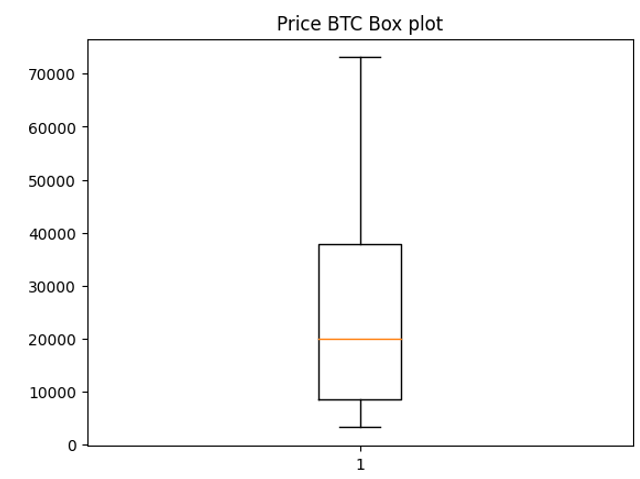
\includegraphics[width=1\textwidth]{bibliography/Figure/BTC_BOXPLOT.png}
    \caption{BTC stock price's boxplot}
    \label{fig:1}
    \end{minipage}
    \hfill
    \begin{minipage}{0.23\textwidth}
    \centering
    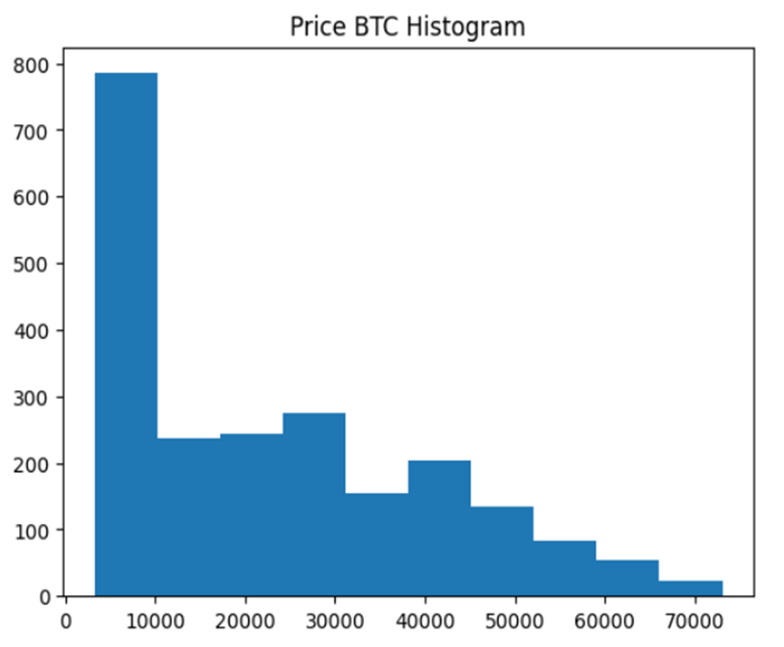
\includegraphics[width=1\textwidth]{bibliography/Figure/BTC_HISTOGRAM.png}
    \caption{BTC stock price's histogram}
    \label{fig:2}
    \end{minipage}
\end{figure}

\begin{figure}[H]
    \centering
    \begin{minipage}{0.23\textwidth}
    \centering
    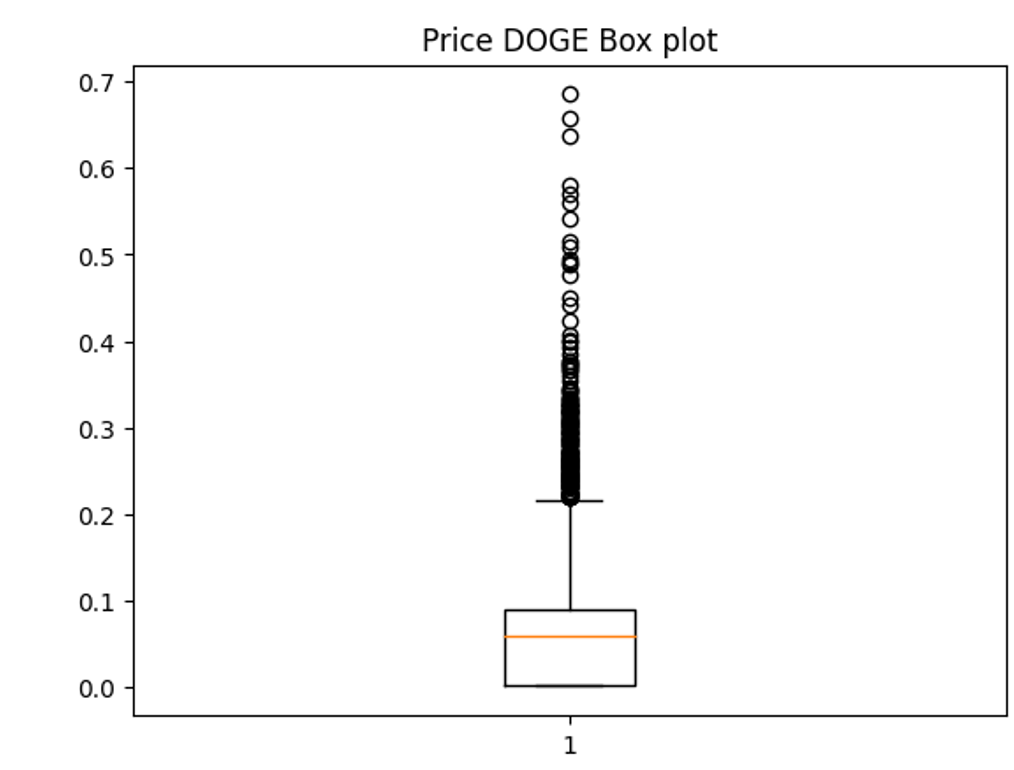
\includegraphics[width=1\textwidth]{bibliography/Figure/DOGE_BOXPLOT.png}
    \caption{DOGE stock price's boxplot}
    \label{fig:1}
    \end{minipage}
    \hfill
    \begin{minipage}{0.23\textwidth}
    \centering
    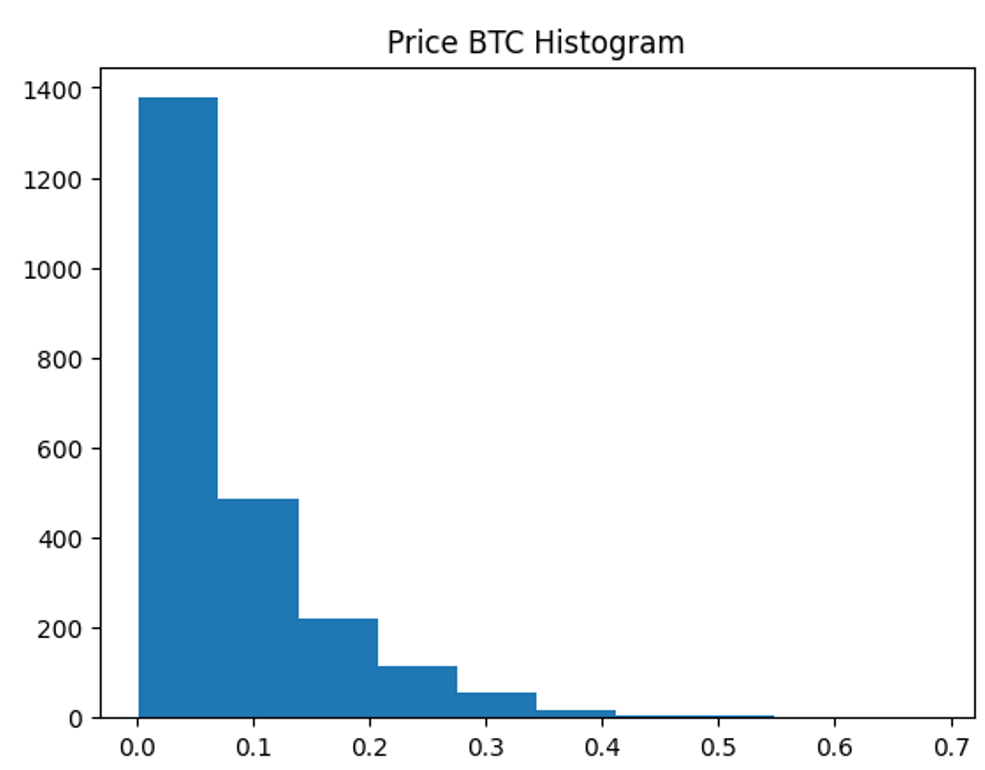
\includegraphics[width=1\textwidth]{bibliography/Figure/DOGE_HISTOGRAM.png}
    \caption{DOGE stock price's histogram}
    \label{fig:2}
    \end{minipage}
\end{figure}

\begin{figure}[H]
    \centering
    \begin{minipage}{0.23\textwidth}
    \centering
    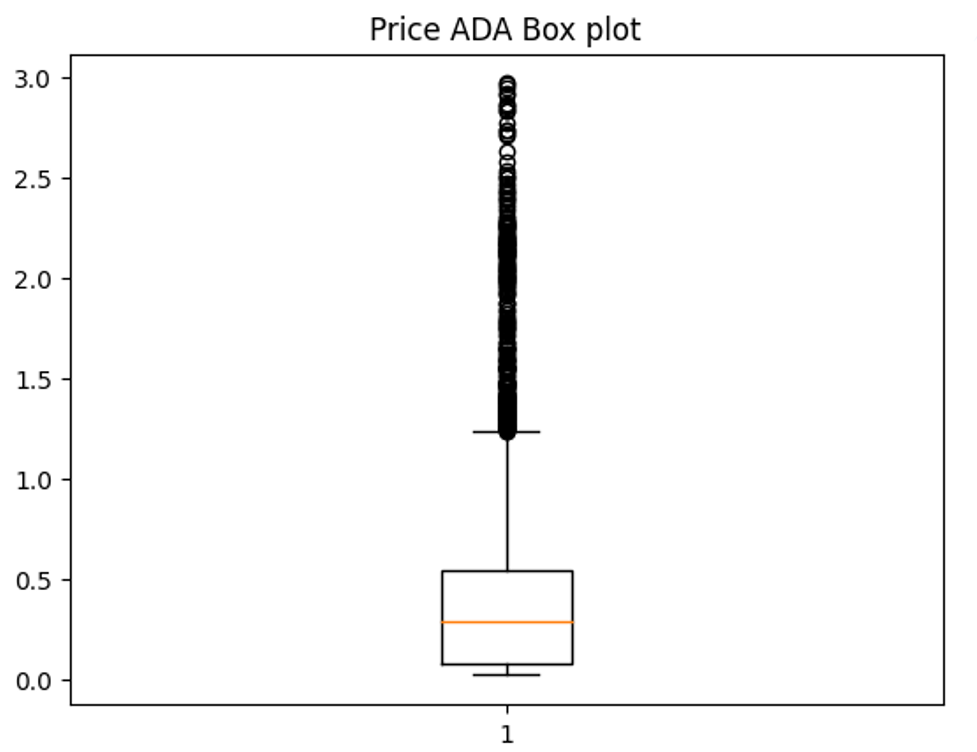
\includegraphics[width=1\textwidth]{bibliography/Figure/ADA_BOXPLOT.png}
    \caption{ADA stock price's boxplot}
    \label{fig:1}
    \end{minipage}
    \hfill
    \begin{minipage}{0.23\textwidth}
    \centering
    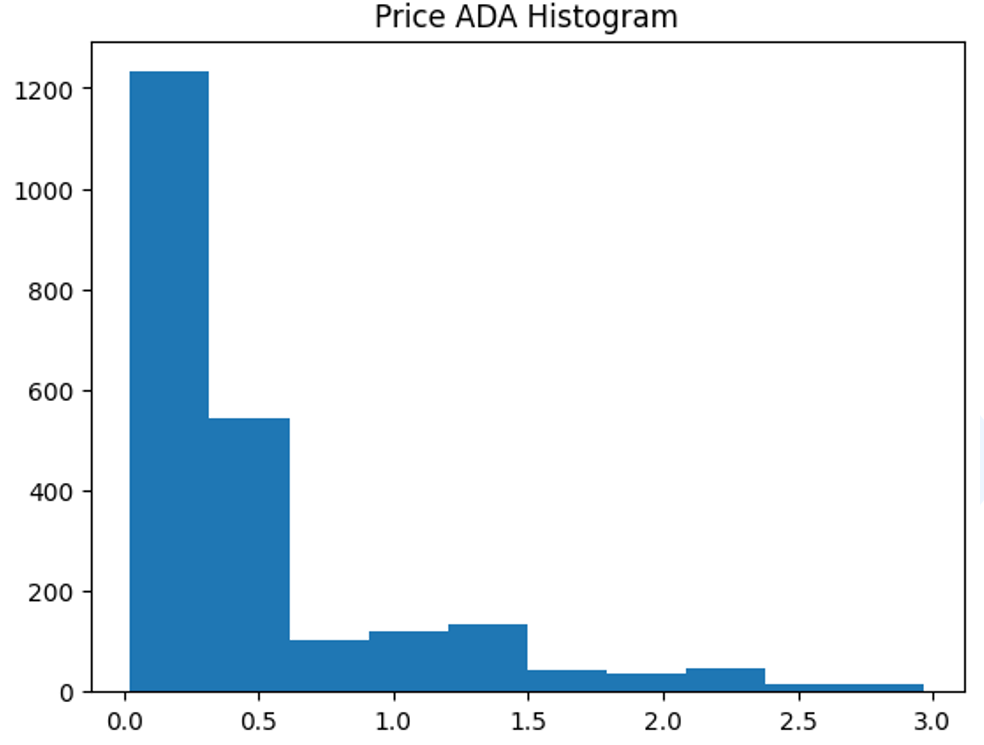
\includegraphics[width=1\textwidth]{bibliography/Figure/ADA_HISTOGRAM.png}
    \caption{ADA stock price's histogram}
    \label{fig:2}
    \end{minipage}
\end{figure}

\section{Methodology}
\subsection{Linear Regression}
Linear regression\cite{b9} is a statistical method used to study the relationship between a dependent variable (target variable) and one or more independent variables (predictor variables). The main objective of regression analysis is to predict or describe the dependent variable based on the independent variables
There are two types of linear regression: 
\newline  Simple Linear Regression: This method establishes a relationship between the dependent variable ((Y)) and a single independent variable ((X)). The simple linear regression equation is:

\[Y=\beta_0+\beta_1X_1+\beta_2X_2+\cdots+\beta_kX_k+\varepsilon\]
Where:\\
	\indent\textbullet\ Y is the dependent variable (Target Variable).\\
	\indent\textbullet\ \(X_1, X_2, \ldots, X_k\) are the independent (explanatory) variables.\\
	\indent\textbullet\ \(\beta_0\) is the intercept term.\\
	\indent\textbullet\ \(\beta_1,..., \beta_k\) are the regression coefficients for the independent variables.\\
	\indent\textbullet\ \(\varepsilon\) is the error term.
\newline Linear regression can be used to predict the value of the dependent variable based on the independent variables. With a defined linear relationship, the regression model can make predictions and estimate values for the future.
 \subsection{Autoregressive Integrated Moving Average (ARIMA)}

The ARIMA\cite{b10} (AutoRegressive Integrated Moving Average) model is one of the fundamental time series forecasting models that utilizes past values and forecast errors of a time series to predict future values.

\textbf{Time Series}: A time series is a sequence of data points collected in chronological order. It represents observations taken at successive time intervals (e.g., daily stock prices, monthly temperature readings, hourly website traffic).

ARIMA integrates two processes: the autoregressive process of order $p$ – AR($p$) and the moving average process of order $q$ – MA($q$). Additionally, differencing integration $I(d)$ (or lag operator) is necessary to transform the time series into a stationary series.

\textbf{Stationary Series}: A time series is said to be stationary if its properties, such as mean, variance, and autocorrelation, do not change over time and it does not exhibit a trend component.

To check for stationarity in a time series, two common tests are used: the Dickey-Fuller test (DF) and the Augmented Dickey-Fuller test (ADF).

\textbf{Autoregressive Process of Order $p$ – AR($p$)}: This process finds the relationship between the current data and $p$ previous data points (lags).

\textbf{Moving Average Process of Order $q$ – MA($q$)}: This process finds the relationship between the current data and $q$ previous forecast errors.

\textbf{Differencing Integration $I(d)$}: This compares the differences between $d$ observations (the difference between the current value and the value $d$ periods ago) to transform a series into a stationary series.

The ARIMA model parameters are defined as follows:

$p$: The number of past values included in the AR model. The AR process can be represented as:
\[
y_t = c + \phi_1 y_{t-1} + \phi_2 y_{t-2} + \cdots + \phi_p y_{t-p} + \epsilon_t
\]
where:
\begin{itemize}
    \item $c$ is a constant
    \item $\phi_1, \ldots, \phi_p$ are the parameters
    \item $\epsilon_t$ is white noise
\end{itemize}

$d$: The number of times the series is differenced.

$q$: The number of past forecast errors in the MA model or the size of the moving average window. The model is termed MA because $y_t$ can be considered a weighted moving average of past forecast errors.

The full ARIMA($p, d, q$) model equation is:
\[
\Phi_p (B) \nabla^d y_t = \Theta_q (B) \epsilon_t
\]
where:
\begin{itemize}
    \item $\nabla^d y_t$ is the $d$th differenced time series
    \item $\Phi_p (B)$ represents the autoregressive part with lag operator $B$
    \item $\Theta_q (B)$ represents the moving average part with lag operator $B$
\end{itemize}

ARIMA models are not universally perfect for all time series data and work best when data is time-dependent and forecasts are point-in-time. Random data often performs poorly with ARIMA models.
 
\subsection{Gated Recurrent Unit (GRU)}
GRUs were developed to address the vanishing gradient problem, a key limitation of traditional RNNs, which hinders their ability to learn long-term dependencies in sequential data. While similar to LSTMs in their use of gates to control information flow, GRUs are a simplified architecture with fewer parameters. They employ update gates and reset gates to selectively remember or forget information from previous time steps, mitigating the vanishing gradient issue and enabling them to capture long-term dependencies more effectively \cite{b11}. The structure of GRU is shown in Fig. 7. 
\begin{figure}[H]
  \centering
  \begin{minipage}{1\linewidth}
    \centering
    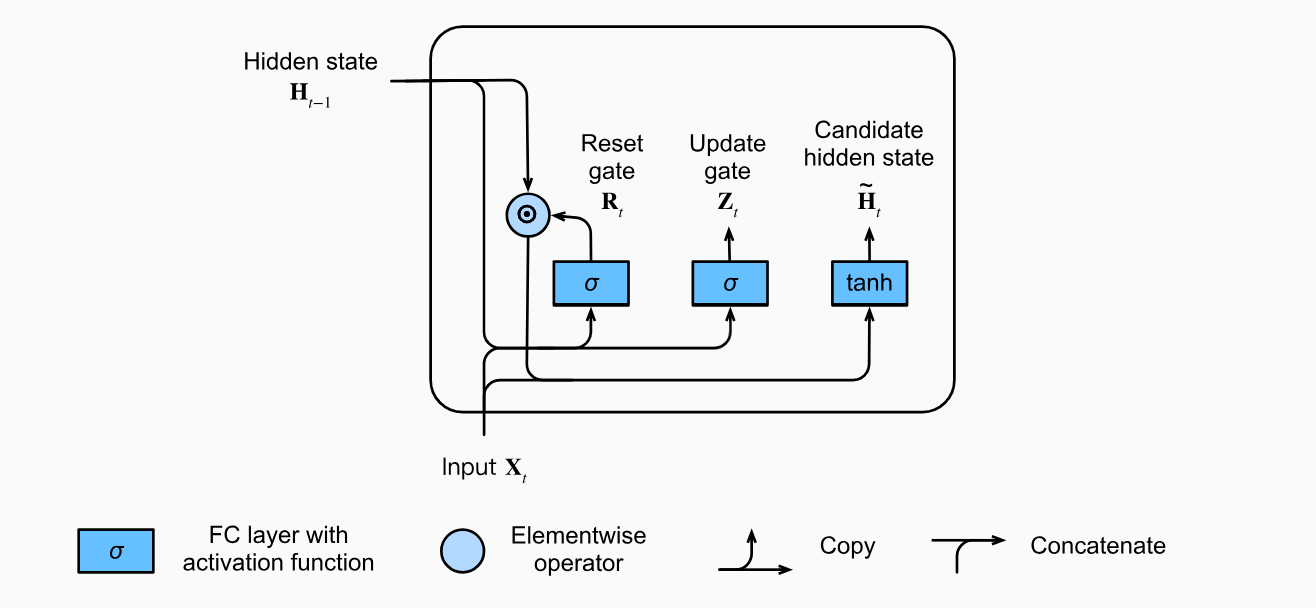
\includegraphics[width=\linewidth]{bibliography/Figure/models/gru_model.png}
    \caption{The structure of a GRU.}
    \label{fig7}
  \end{minipage}
\end{figure}
\textbf{Reset Gate and Update Gate Model}: The reset gate controls how much of the previous state we want to remember. Similarly, the update gate controls how much of the new state is simply a copy of the old state. Mathematically, at a given time step \( t \), assuming the input is a mini-batch \( X_t \in \mathbb{R}^{n \times d} \) (number of examples: \( n \), number of inputs: \( d \)) and the hidden state from the previous time step is \( H_{t-1} \in \mathbb{R}^{n \times h} \) (number of hidden units: \( h \)), the reset gate \( R_t \in \mathbb{R}^{n \times h} \) and update gate \( Z_t \in \mathbb{R}^{n \times h} \) are calculated as follows \cite{b12}:
\[
R_t = \sigma(X_t W_{xr} + H_{t-1} W_{hr} + b_r),
\]
\[
Z_t = \sigma(X_t W_{xz} + H_{t-1} W_{hz} + b_z)
\]
Where:
\begin{itemize}
  \item \( W_{xr}, W_{xz} \in \mathbb{R}^{d \times h} \), \( W_{hr}, W_{hz} \in \mathbb{R}^{h \times h} \): The weight parameters.
  \item \( b_r, b_z \in \mathbb{R}^{1 \times h} \): The bias parameters.
\end{itemize}
\textbf{Candidate Hidden State Model}: Integrating the reset gate \( R_t \), we arrive at the candidate hidden state \( \tilde{H}_t \) at time step \( t \):
\[
\tilde{H}_t = \tanh(X_t W_{xh} + (R_t \odot H_{t-1}) W_{hh} + b_h)
\]
Where:
\begin{itemize}
  \item \( W_{xh} \in \mathbb{R}^{d \times h} \), \( W_{hh} \in \mathbb{R}^{h \times h} \): The weight parameters.
  \item \( b_h \in \mathbb{R}^{1 \times h} \): The bias, and \( \odot \) represents the Hadamard (element-wise) product operator.
\end{itemize}
\textbf{Hidden State Model}: Combining the effect of the update gate \( Z_t \), we determine the extent to which the new hidden state \( H_t \in \mathbb{R}^{n \times h} \) aligns with the old state \( H_{t-1} \) compared to its resemblance to the new candidate state \( \tilde{H}_t \). The update gate \( Z_t \) can be used for this purpose, simply by employing clever element-wise convex combinations of \( H_{t-1} \) and \( \tilde{H}_t \). This leads to the final update equation for GRU:
\[
H_t = Z_t \odot H_{t-1} + (1 - Z_t) \odot \tilde{H}_t
\] 
\textbf{GRUs have two distinguishing features}: The reset gate, which captures short-term dependencies in the sequence, and the update gate, which captures long-term dependencies in the sequence.

\subsection{Recurrent Neural Network (RNN)}
Recurrent Neural Network (RNN) acts like a specialized brain for handling sequences, whether they are sentences or time-based data. Imagine it as a smart cell with own memory, understanding each element and retaining context. This memory capability allows an RNN to effectively capture patterns and relationships within sequences, making RNN well-suited for predicting future values in time series data such as stock prices or weather conditions, where historical information is essential for accurate forecasts \cite{b13}.\\
RNN is characterized by recurrent connections that allow information to flow from one time step to the next. At each step, it takes an input, updates its internal state, and produces an output based on previous inputs, effectively using this state as a memory to influence future processing \cite{b14}.\\
\begin{figure}[H]
  \centering
  \begin{minipage}{0.5\linewidth}
    \centering
    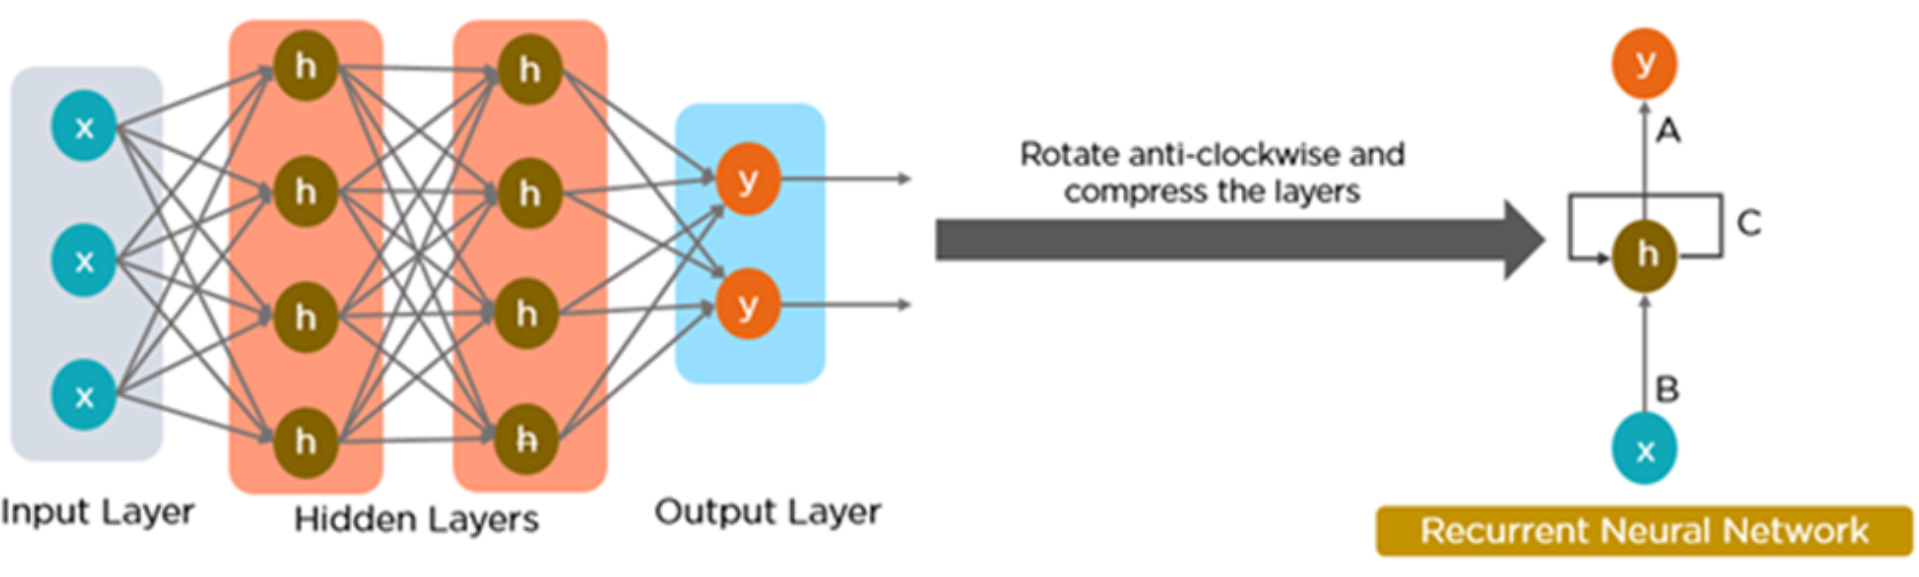
\includegraphics[width=\linewidth]{bibliography/Figure/models/RNN.png}
    \caption{RNN's architecture}
    \label{fig8}
  \end{minipage}
\end{figure}
Here, the input layer (x) receives the initial element of the sequence data. The hidden layer (h) comprises interconnected neurons that process the current input along with information from the previous hidden layer's state, capturing the network's memory of past inputs and understanding the current element in context. The output layer (y) is responsible for generating the network's prediction based on the processed information.\\
At any given time \( t \), \( h_t \) can be computed using the following formula:
\[
h_t = f_w(h_{t-1}, x_t)
\]
Where:
\begin{itemize}
  \item \( h_t \): The hidden state at time step \( t \).
  \item \( h_{t-1} \): Previous hidden state from time step \( t-1 \).
  \item \( x_t \): Input at time step \( t \).
  \item \( f_w \): Function with parameters \( w \), typically an activation function.
\end{itemize}
The output of the Recurrent Neural Network (RNN) at time step \( t \) is calculated by the following formula:
\[
y_t = W_{hy} \cdot h_t
\]
Where:
\begin{itemize}
\item \( y_t \): The output at time step \( t \).
  \item \( W_{hy} \): The weight matrix between the hidden state and the output.
  \item \( h_t \): The hidden state at time step \( t \).
\end{itemize}
Traditional Recurrent Neural Networks (RNNs) struggle with long sequences due to the "vanishing gradients" problem, where important gradients diminish over time, hampering learning and prediction accuracy. To address this, advanced models like LSTM and GRU have been developed. These models use sophisticated mechanisms to selectively retain and update information, enhancing their ability to capture long-term dependencies in sequential data \cite{b16}.

\subsection{Long Short-Term Memory (LSTM)}
Long Short-Term Memory (LSTM) is a specialized type of Recurrent Neural Network designed to capture long-term dependencies in sequential data like time series, text, and speech. LSTM uses a memory cell and gates—input, forget, and output—to manage information flow, selectively retaining or discarding information to address the vanishing gradient problem in traditional RNN. LSTMs find wide application in natural language processing, speech recognition, and time series forecasting \cite{b15}.\\
A standard LSTM unit comprises a memory cell and three gates:
\begin{itemize}
    \item The cell retains information across time intervals.
    \item The input gate controls which information enters the cell.
    \item The forget gate determines what information to discard from the cell.
    \item The output gate decides which information to use for output.
\end{itemize}
These gates use sigmoid functions to generate outputs between 0 and 1 and are trained using backpropagation algorithms.
\begin{figure}[H]
  \centering
  \begin{minipage}{0.5\linewidth}
    \centering
    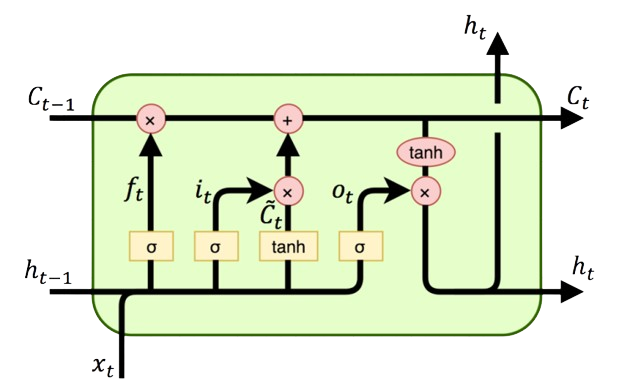
\includegraphics[width=\linewidth]{bibliography/Figure/models/LSTM.png}
    \caption{At time step t of the LSTM model}
    \label{fig9}
  \end{minipage}
\end{figure}
\textbf{Forget gate}: The forget gate in LSTM is crucial for deciding which information should be discarded from the cell state. This decision is determined by a sigmoid layer known as the "forget gate layer." It evaluates \( h_{t-1} \) (previous hidden state) and \( x_t \) (current input) to generate values between 0 and 1 for each element in the cell state \( C_{t-1} \):
\[
f_t = \sigma(W_f \cdot [h_{t-1}, x_t] + b_f)
\]
Where:
\begin{itemize}
  \item \( f_t \): The forget gate output at time step \( t \).
  \item \( \sigma \): The sigmoid activation function.
  \item \( W_f \): The weight parameters connecting \( h_{t-1} \) and \( x_t \) to the forget gate.
  \item \( b_f \): The bias vector.
  \item \( [h_{t-1}, x_t] \): The concatenation of \( h_{t-1} \) and \( x_t \).
\end{itemize}
\textbf{Input gate}: Firstly, a sigmoid layer known as the "input gate layer" determines which values will be updated
\[
i_t = \sigma(W_i \cdot [h_{t-1}, x_t] + b_i)
\]
Where:
\begin{itemize}
  \item \( i_t \): The vector of input gate values for the current time step.
  \item \( \sigma \): The sigmoid activation function.
  \item \( W_i \): The weight parameters connecting \( h_{t-1} \) and \( x_t \) to the input gate.
  \item \( b_i \): The bias vector specific to the input gate.
  \item \( [h_{t-1}, x_t] \): The concatenation of the previous hidden state and the current input.
\end{itemize}
Secondly, a tanh layer generates a vector of new candidate values, \( \tilde{C}_t \), which could potentially be added to the state. These two components are then integrated to form an updated state:
\[
\tilde{C}_t = \tanh(W_C \cdot [h_{t-1}, x_t] + b_C)
\]
where:
\begin{itemize}
  \item \( \tilde{C}_t \): The vector of new candidate values.
  \item \( \tanh \): The hyperbolic tangent activation function.
  \item \( W_C \): The weight parameters connecting \( h_{t-1} \) and \( x_t \) to the tanh layer.
  \item \( b_C \): The bias vector.
\end{itemize}
It's time to update the old cell state \( C_{t-1} \) to the new cell state \( C_t \). Multiply the old cell state \( C_{t-1} \) by the forget gate output \( f_t \) to discard the information decided for forgetting. Then add the new candidate values, scaled by the input gate output \( i_t \), for each state value:
\[
C_t = f_t \cdot C_{t-1} + i_t \cdot \tilde{C}_t
\]
Where:
\begin{itemize}
  \item \( C_{t-1} \): The previous cell state.
  \item \( C_t \): The updated cell state.
  \item \( f_t \): The forget gate output.
  \item \( i_t \): The input gate output.
  \item \( \tilde{C}_t \): The new candidate cell state.
\end{itemize}
\textbf{Output gate}: This output is derived from the cell state but is filtered. Initially, a sigmoid layer determines which components of the cell state to the output.
\[
o_t = \sigma(W_o \cdot [h_{t-1}, x_t] + b_o)
\]
Where:
\begin{itemize}
  \item \( o_t \): The output gate output at time step \( t \).
  \item \( \sigma \): The sigmoid activation function.
  \item \( W_o \): The weight parameters connecting \( h_{t-1} \) and \( x_t \) to the output gate.
  \item \( b_o \): The bias vector specific to the output gate.
  \item \( [h_{t-1}, x_t] \): The concatenation of the previous hidden state and the current input.
\end{itemize}
Then, the cell state undergoes transformation through the tanh function, scaling the values to a range between -1 and 1. Subsequently, it is multiplied by the output of the sigmoid gate, ensuring that only selected components are outputted \cite{b17}.
\[
h_t = o_t \cdot \tilde{h}_t
\]
Where:
\begin{itemize}
  \item \( \tilde{h}_t \): The new hidden state at time step \( t \).
  \item \( C_t \): The cell state at time step \( t \).
  \item \( o_t \): The output gate output at time step \( t \).
  \item \( \tanh \): The hyperbolic tangent activation function.
\end{itemize}
\subsection{Hybrid Models}
Hybrid models in artificial intelligence integrate different machine-learning techniques to enhance prediction performance and accuracy. By combining features from various models and algorithms, these models leverage their strengths while minimizing their weaknesses. Hybrid models are particularly useful in applications involving multiple data sources or types, such as medical data analytics, financial analytics, and marketing analytics.\\
Time series data can be conceptualized as an additive combination of trend, seasonal effects, cycles, and random error (residuals), represented by the equation:
\[
series = trend + season + cycle + error
\]
In this model, each term is considered a component of the time series. The residuals are the differences between the target values and the model's predictions, representing the deviation between the actual data curve and the fitted curve.\\
When constructing hybrid models, it is common to use a simple learning algorithm, often linear, followed by a complex, non-linear learner such as Gradient Boosted Decision Trees (GBDTs) or deep neural networks. The simple model typically serves as a "helper" to the more powerful algorithm, enhancing its performance and effectiveness. This strategy has proven to be the most practical and effective approach in many applications \cite{b18}.\\
Hybrid models amalgamate diverse machine-learning techniques to significantly enhance the accuracy of stock price forecasting. Specifically, for predicting closing prices, the hybrid model employs the following methodologies:\\
\textbf{Linear Regression for Trend Modeling}:
Utilizes linear regression to capture the long-term trend in closing prices. The trend component portrays the overarching direction of the stock price series over time, discerning whether it exhibits growth, decline, or stability.\\
\textbf{Exponential Smoothing for Seasonality}: Applies Exponential Smoothing to model seasonal components inherent in the stock price data. Seasonality encompasses repetitive patterns such as daily, weekly, or monthly fluctuations, which exert influence on stock prices.\\
\textbf{XGBoost for Residual Analysis}: Detrends the data by removing both the identified trend and seasonal components. Utilizes XGBoost, a potent gradient boosting algorithm, to model the residual errors that persist after detrending. This step captures intricate, non-linear relationships and anomalies in the residual errors of the stock price series.
Finally, the model integrates predictions from the trend, seasonal, and residual components to generate future stock price forecasts. This comprehensive approach ensures robust forecasting accuracy, enabling informed financial decision-making in dynamic and volatile markets.
\subsection{AR-EMOS}

Ensemble Model Output Statistics (EMOS)\cite{b20} is a widely used statistical method to improve the accuracy of weather forecasts by combining multiple forecasts from different models. The AR-EMOS (Autoregressive EMOS)\cite{b21} model extends the EMOS approach by integrating an autoregressive (AR) process to adjust the forecasts. In this report, we will apply the AR-EMOS model to predict cryptocurrency prices, a field that requires high accuracy and the ability to handle complex fluctuations.


\textbf{Basic Ensemble Model Output Statistics (EMOS)}

Assumption: Assume that the cryptocurrency price at time $t$ follows a normal distribution:
\[
Y(t) \mid x_1(t), \ldots, x_m(t) \sim N(\mu(t), \sigma^2(t))
\]
where $Y(t)$ is the observed price, and $x_1(t), \ldots, x_m(t)$ are the forecasts from different models.

Predictive Mean ($\mu(t)$) and Predictive Variance ($\sigma^2(t)$): These are linked to the ensemble forecasts via the formulas:
\[
\mu(t) := a_0 + a_1 \bar{x}(t)
\]
\[
\log(\sigma(t)) := b_0 + b_1 \log(s(t))
\]
where $\bar{x}(t)$ is the ensemble mean, and $s(t)$ is the empirical ensemble standard deviation at time $t$. The coefficients $a_0, a_1, b_0, b_1$ are estimated by minimizing a proper scoring rule, typically the Continuous Ranked Probability Score (CRPS).

\textbf{Autoregressive EMOS (AR-EMOS)}

The AR-EMOS model incorporates autoregressive elements into the forecast adjustment process:

\textbf{AR Error Series}: The error $r_k(t)$ between the observed price and the forecast from each model is modeled as an AR process of order $p_k$:
\[
r_k(t) := Y(t) - x_k(t)
\]

\textbf{AR-Adjusted Forecast Ensemble}: The AR-adjusted forecasts are obtained via:
\[
\tilde{x}_k(t) := x_k(t) + \hat{r}_k(t) = x_k(t) + \eta_k + \sum_{j=1}^{p_k} \tau_{k,j} (\hat{r}_k(t-j) - \eta_k)
\]
where $\eta_k, \tau_{k,j}$ are the AR model coefficients, and $\hat{r}_k(t)$ are the estimated residuals.

\textbf{Predictive Mean ($\mu(t)$) and Predictive Variance ($\sigma(t)$)}:
\[
\mu(t) := \frac{1}{m} \sum_{k=1}^{m} \tilde{x}_k(t)
\]
\[
\sigma(t) := \omega \sigma_1(t) + (1 - \omega) \sigma_2(t)
\]
where $\sigma_1(t)$ is the empirical variance of the AR process, and $\sigma_2(t)$ is the empirical standard deviation of the AR-adjusted forecasts. The weight $\omega$ is determined by minimizing the CRPS of the predictive Gaussian distribution.

\textbf{Conclusion}

The AR-EMOS model not only leverages the power of multiple forecasts but also utilizes autoregressive processes to adjust errors, resulting in more accurate forecasts. Applying AR-EMOS in predicting cryptocurrency prices can better capture the complex market fluctuations, thus supporting more effective investment decisions.
\subsection{FEDformer}
FEDformer's innovative combination of Transformer with seasonal-trend decomposition to enhance long-term series forecasting by capturing both the global profile of time series and detailed structures. The method renovates the Transformer architecture by introducing components such as the Frequency Enhanced Block (FEB), Frequency Enhanced Attention (FEA), and the Mixture Of Experts Decomposition block (MOEDecomp) \cite{b22}. The model follows the encoder-decoder architecture proposed by Vaswani et al. (2017) \cite{b23}, incorporating a multi-head attention mechanism for effective modeling of dependencies. The structure of FEDformer is shown in Fig. 10.
\begin{figure}[H]
  \centering
  \begin{minipage}{1\linewidth}
    \centering
    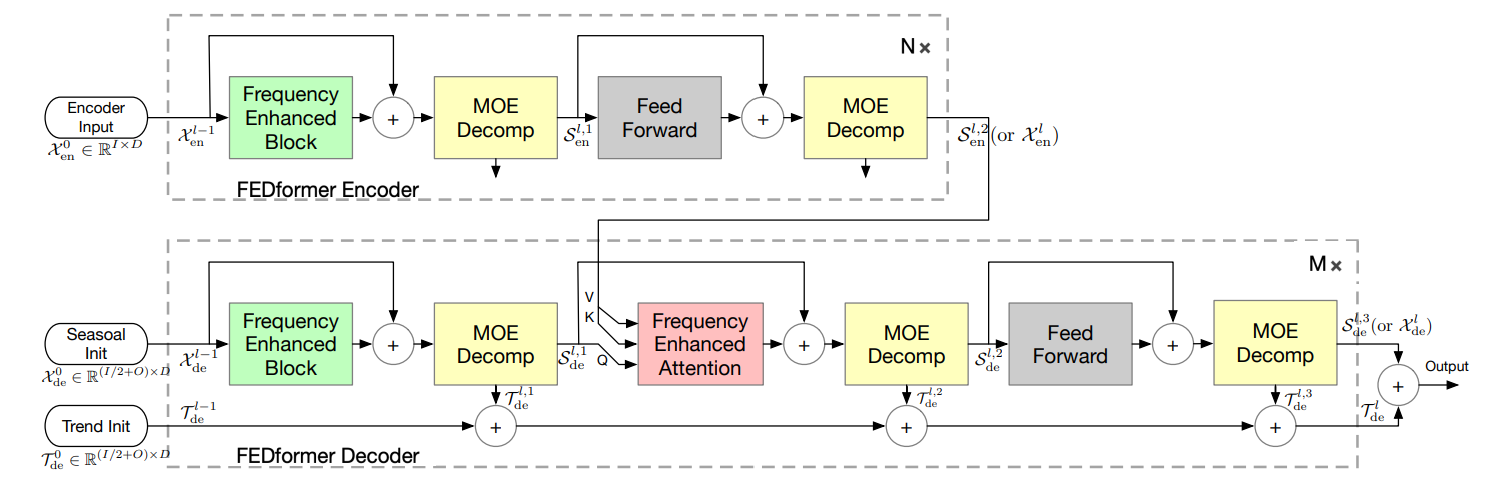
\includegraphics[width=\linewidth]{bibliography/Figure/models/fedformer.png}
    \caption{The structure of FEDformer }
    \label{fig9}
  \end{minipage}
\end{figure}

\textbf{The Frequency Enhanced Block (FEB)} leverages sparse representations of time series using the Fourier basis, selecting a subset of frequency components for a more comprehensive representation. This approach retains crucial information about trend changes, improving forecasting accuracy.

\textbf{The Frequency Enhanced Attention (FEA) and MOEDecomp} facilitate improved modeling of long-term dependencies and seasonal-trend decomposition, respectively. By integrating these components into the Transformer framework, FEDformer optimally combines seasonal-trend decomposition and Transformer strengths for enhanced forecasting performance on long-term time series data.

\section{Result}
\subsection{Evaluation Methods}
\textbf{Mean Absolute Percent Error} (MAPE): A measure commonly used to assess the performance or accuracy of predictive models is Mean Absolute Percentage Error (MAPE). It calculates the average percentage difference between the actual values and the predicted values.\\
\[
\text{MAPE} = \frac{1}{m} \sum_{i=1}^{m} \left| \frac{Y_i - X_i}{Y_i} \right|
\]\\
\textbf{Root Mean Squared Error} (RMSE): A measure of the performance or accuracy of a predictive model measured by calculating the square root of the mean square error between the predicted values and the actual values.\\
\[
\text{RMSE} = \sqrt{\frac{1}{m} \sum_{i=1}^{m} (X_i - Y_i)^2}
\]
\\
\textbf{Mean Absolute Error} (MAE): A measure of a predictive model's performance or accuracy measured by averaging the absolute value of the error between the actual value and the predicted value.\\
\[
\text{MAE} = \frac{1}{m} \sum_{i=1}^{m} |X_i - Y_i|
\]

\subsection{BTC Dataset} 
\begin{table}[H]
    \centering
    \begin{tabular}{|>{\centering\arraybackslash}p{1.1cm}|>{\centering\arraybackslash}p{1.8cm}|>{\centering\arraybackslash}p{1cm}|>{\centering\arraybackslash}p{1.35cm}|>{\centering\arraybackslash}p{1.25cm}|}
         \hline
         \multicolumn{5}{|c|}{\textbf{Dataset's Evaluation}}\\
         \hline
         Model & Training:Testing & MAE & RMSE & MAPE\\
         \hline
         \multirow{3}{*}{LN} & 7:3 & 23106.05 & 620051055 & 93.02 \\ & 8:2 & 12309.19 & 184845175 & 35.18 \\ & \textbf{9:1} & \textbf{13052.26} & \textbf{285307317} & \textbf{21.8777}\\
         \hline
         \multirow{3}{*}{ARIMA} & 7:3 & 13141.36 & 386545353 & 30.63 \\ & 8:2 & 16316.99 & 496929012 & 33.44 \\ & \textbf{9:1} & \textbf{23196.43} & \textbf{710699778} & \textbf{41.021}\\
         \hline
         \multirow{3}{*}{GRU} & 7:3 & 32630.53 & 35951.35 & 7820766.85 \\ &  8:2 & 39640.56 & 42394.117 & 7717808.65 \\ & \textbf{9:1} & \textbf{51151.010} & \textbf{52756.28} & \textbf{7424441.25}\\
         \hline
        \multirow{3}{*}{RNN} & \textbf{7:3} & \textbf{33285.01} & \textbf{36624.1} & \textbf{7985661.9} \\ 
        & 8:2 & 39408.2 & 42174.7 & 7665900.6 \\ 
        & 9:1 & 51311.7 & 52919 & 7447792.4 \\
        \hline
        \multirow{3}{*}{LSTM} & \textbf{7:3} & \textbf{32994.87} & \textbf{36272.19} & \textbf{7923743.27} \\ 
        & 8:2 & 39360.81 & 42060.82 & 7667680.63 \\ 
        & 9:1 & 51679.20 & 53279.30 & 7504225.35 \\
        \hline
         \multirow{3}{*}{\shortstack{HYBRID \\ MODELS}} & 7:3 & 0.0115 & 0.0178 & 2.7661\\ & \textbf{8:2} & \textbf{0.0131}	& \textbf{0.0210} & \textbf{2.2552}\\ & 9:1 & 0.0175 & 0.0257& 2.3920\\
         \hline
         \multirow{3}{*}{AR-EMOS} & 7:3 &  10027.27 & 261245890.7 & 23.589 \\ & 8:2 & 14618.61 & 424866726.9 & 29.244 \\ & \textbf{9:1} &  \textbf{22919.84} &	\textbf{694618434} & 	\textbf{40.5198} \\
         \hline
         \multirow{3}{*}{\shortstack{FED \\ FORMER}} & 7:3 & 45693.13 &  55652.14 &  137.3864 \\ & \textbf{8:2} & \textbf{19144.68} &  \textbf{26880.917} &  \textbf{39.2247} \\ & 9:1 & 25096.88 & 27791.626 & 45.5814\\
         \hline
    \end{tabular}
    \caption{BTC Dataset's Evaluation}
    \label{mbbresult}
\end{table}
\begin{figure}[H]
    \centering
    \begin{minipage}{0.23\textwidth}
    \centering
    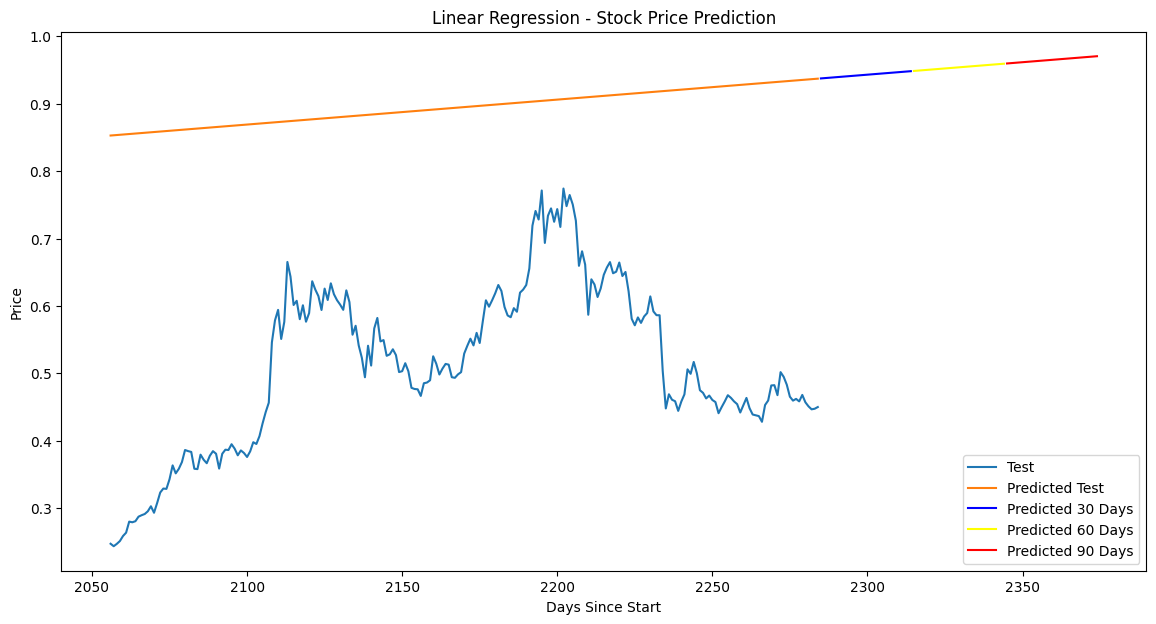
\includegraphics[width=1\textwidth]{bibliography/Figure/LINEAR_ADA_9-1.png}
    \caption{Linear model's result with 9:1 splitting proportion}
    \label{fig10}
    \end{minipage}
    \hfill
    \begin{minipage}{0.23\textwidth}
    \centering
    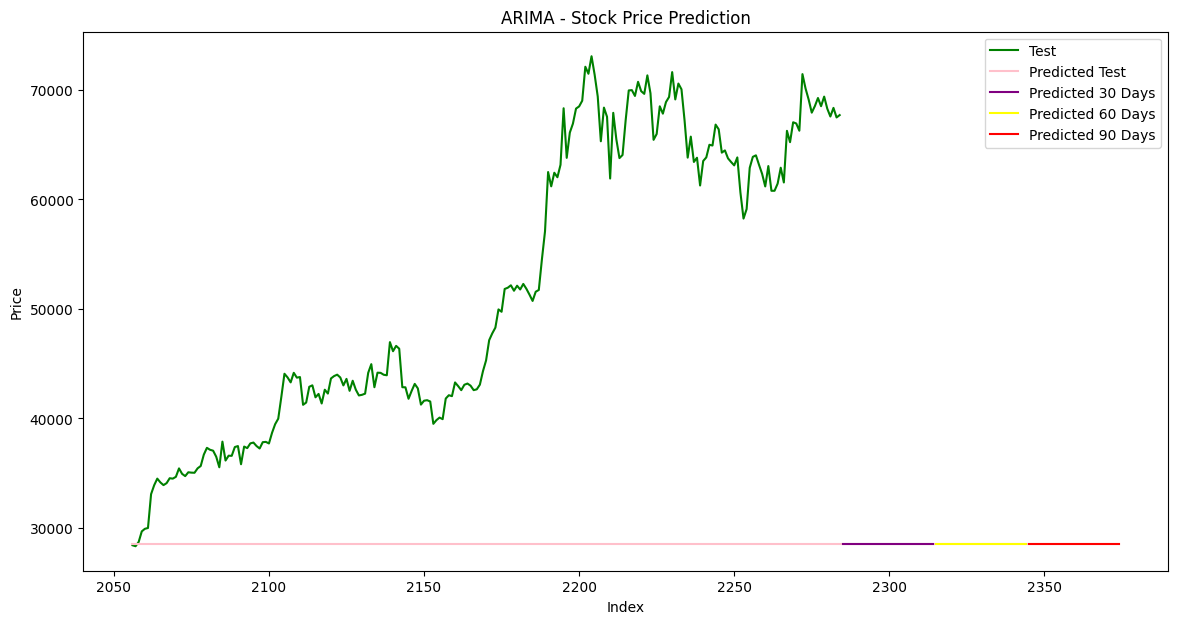
\includegraphics[width=1\textwidth]{bibliography/Figure/PREDICT/BTC_ARIMA_9-1.png}
    \caption{ARIMA model's result with 9:1 splitting proportion}
    \label{fig11}
    \end{minipage}
\end{figure}

\begin{figure}[H]
    \centering
    \begin{minipage}{0.23\textwidth}
    \centering
    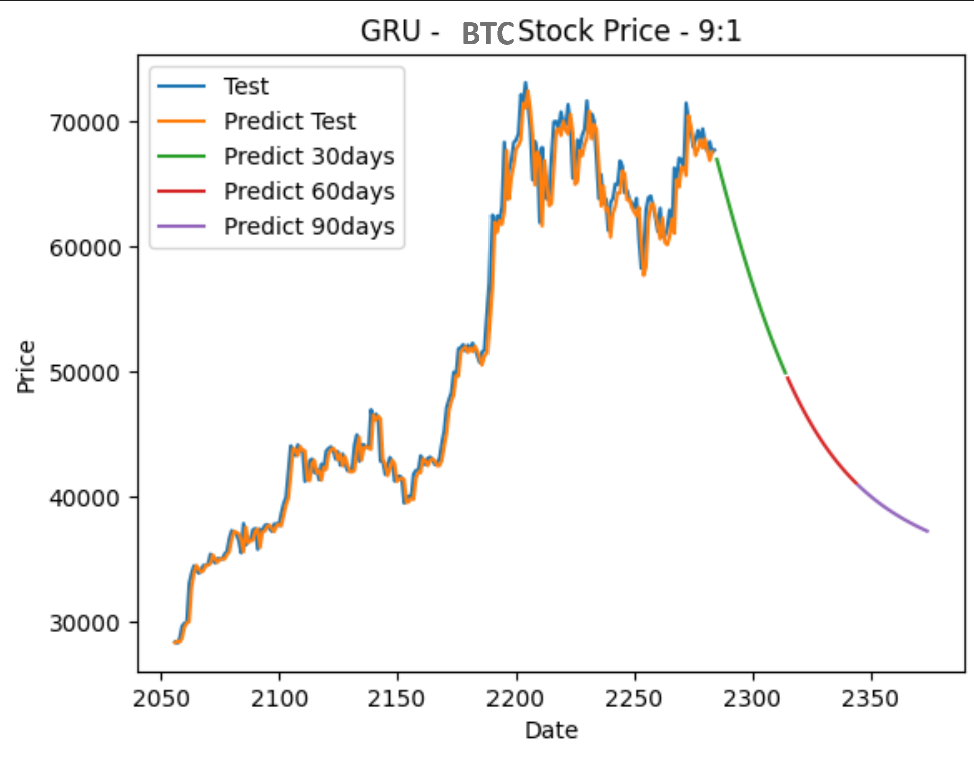
\includegraphics[width=1\textwidth]{bibliography/Figure/GRU btc 91.png}
    \caption{GRU model's result with 9:1 splitting proportion}
    \label{fig10}
    \end{minipage}
    \hfill
    \begin{minipage}{0.23\textwidth}
    \centering
    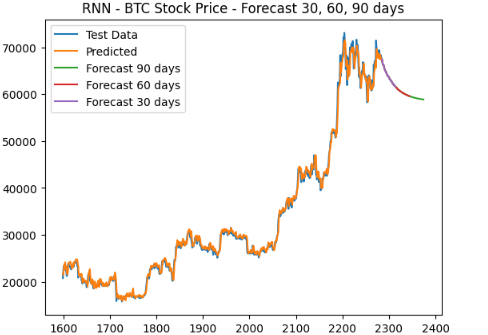
\includegraphics[width=1\textwidth]{bibliography/Figure/PREDICT/RNN/RNN-7-3-BTC.png}
    \caption{RNN model's result with 7:3 splitting proportion}
    \label{fig11}
    \end{minipage}
\end{figure}

\begin{figure}[H]
    \centering
    \begin{minipage}{0.23\textwidth}
    \centering
    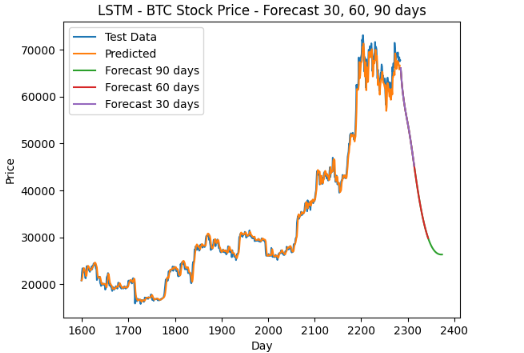
\includegraphics[width=1\textwidth]{bibliography/Figure/PREDICT/LSTM/LSTM-7-3-BTC.png}
    \caption{LSTM model's result with 7:3 splitting proportion}
    \label{fig10}
    \end{minipage}
    \hfill
    \begin{minipage}{0.23\textwidth}
    \centering
    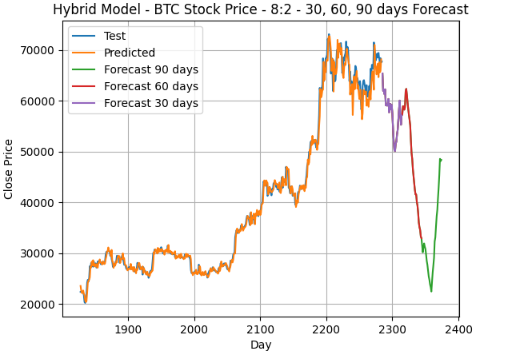
\includegraphics[width=1\textwidth]{bibliography/Figure/PREDICT/HYBRID MODELS/HB-8-2-BTC.png}
    \caption{Hybrid Models's result with 8:2 splitting proportion}
    \label{fig11}
    \end{minipage}
\end{figure}

\begin{figure}[H]
    \centering
    \begin{minipage}{0.23\textwidth}
    \centering
    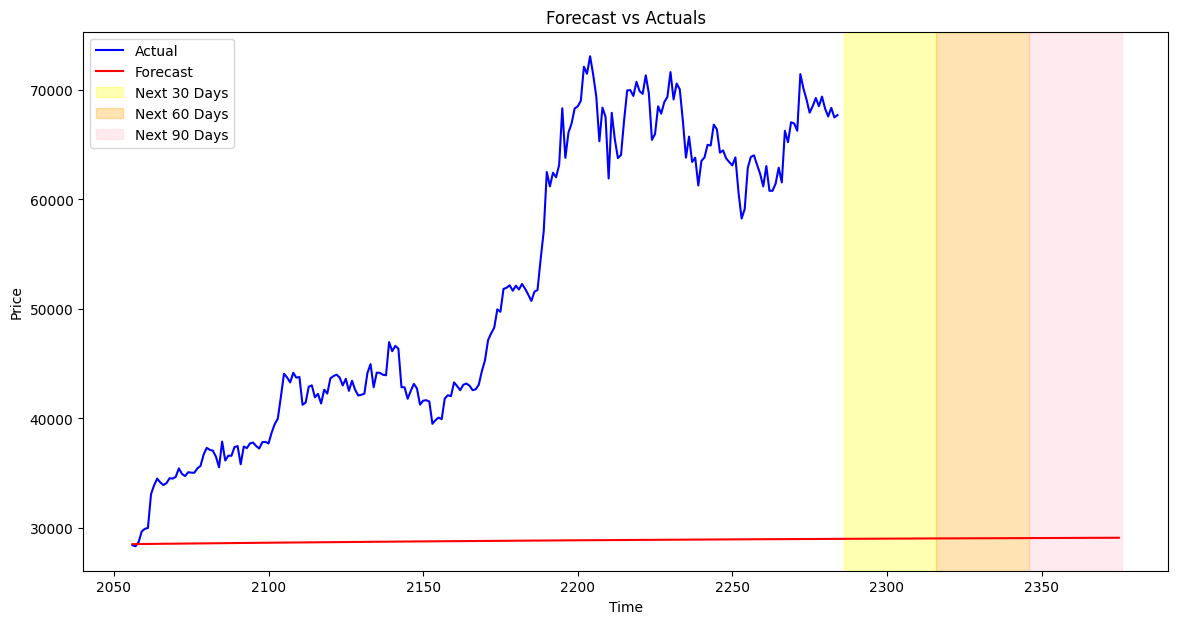
\includegraphics[width=1\textwidth]{bibliography/Figure/PREDICT/BTC_AR-EMOS_9-1.png}
    \caption{AR-EMOS model's result with 9:1 splitting proportion}
    \label{fig10}
    \end{minipage}
    \hfill
    \begin{minipage}{0.23\textwidth}
    \centering
    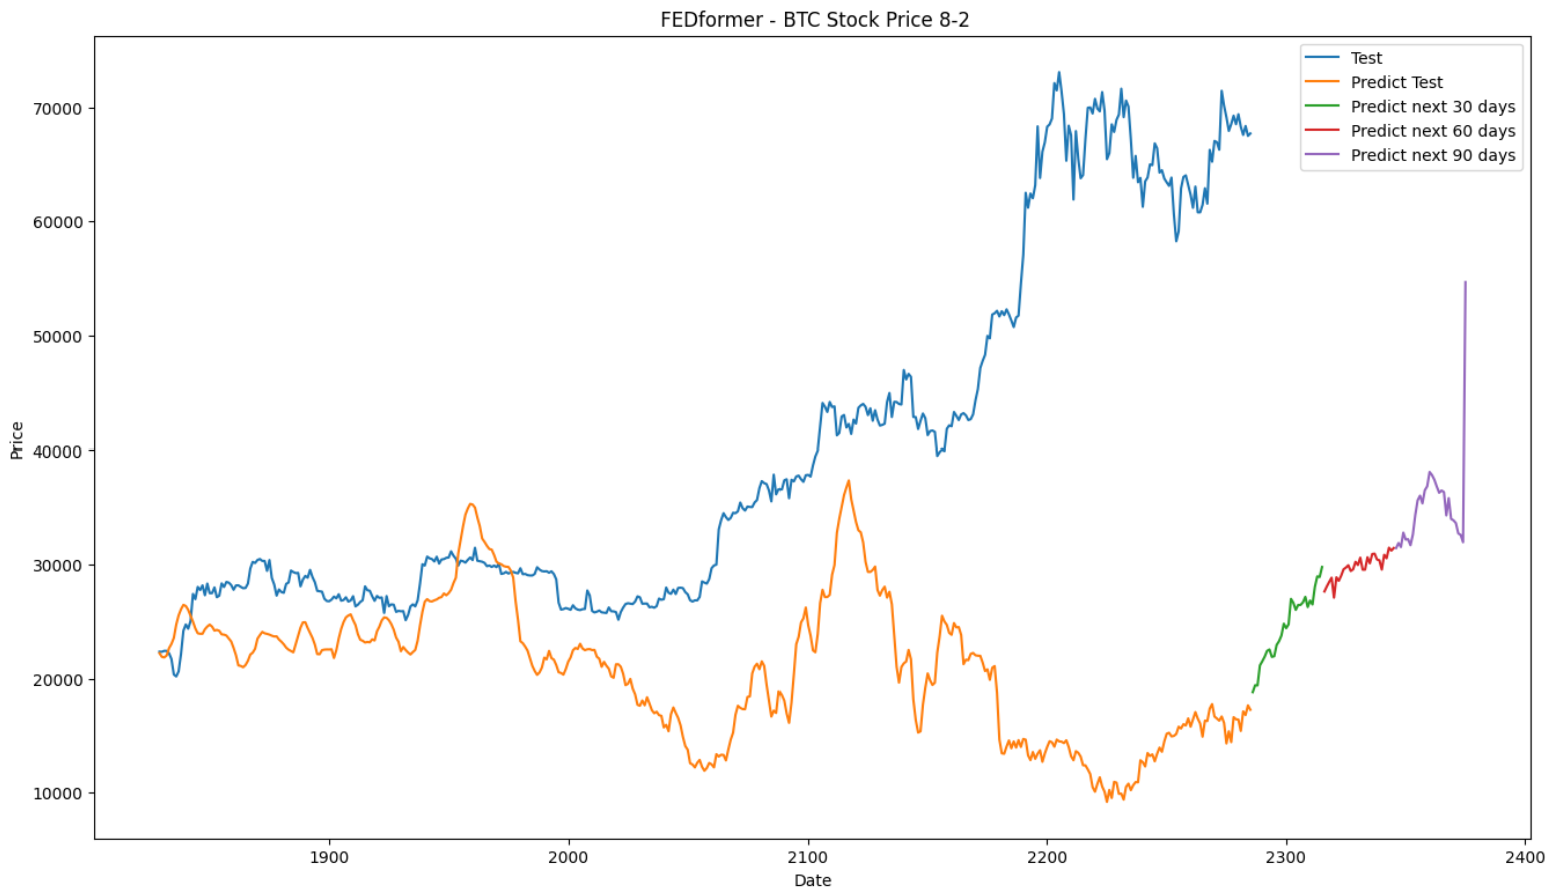
\includegraphics[width=1\textwidth]{bibliography/Figure/FED btc 82.png}
    \caption{FEDFORMER model's result with 8:2 splitting proportion}
    \label{fig11}
    \end{minipage}
\end{figure}


\subsection{DOGE dataset} 
\begin{table}[H]
    \centering
    \begin{tabular}{|>{\centering\arraybackslash}p{1.1cm}|>{\centering\arraybackslash}p{1.8cm}|>{\centering\arraybackslash}p{1cm}|>{\centering\arraybackslash}p{1.3cm}|>{\centering\arraybackslash}p{1cm}|}
         \hline
         \multicolumn{5}{|c|}{\textbf{Dataset's Evaluation}}\\
         \hline
         Model & Training:Testing & MAE & RMSE & MAPE\\
         \hline
         \multirow{3}{*}{LN} & 7:3 & 0.1374 & 0.0197 & 177.24 \\ & 8:2 & 0.0869 & 0.0084 & 114.16 \\ & \textbf{9:1} & \textbf{0.0435} & \textbf{0.00256} & \textbf{50.28} \\
         \hline
         \multirow{3}{*}{ARIMA} & 7:3 & 0.02479 & 0.00165 & 21.55 \\ & 8:2 & 0.0246 & 0.0016 & 21.10 \\ & \textbf{9:1} & \textbf{0.0554} & \textbf{0.0048} & \textbf{41.147}\\
         \hline
         \multirow{3}{*}{GRU} & 7:3 & 0.03526 &  0.03906 & 27.4560 \\ &  \textbf{8:2} & \textbf{0.03640} & \textbf{0.04097} & \textbf{26.6066} \\ & 9:1 & 0.05293 & 0.05749 & 31.588\\
         \hline
         \multirow{3}{*}{RNN} & \textbf{7:3} & \textbf{0.0344} & \textbf{0.0378} & \textbf{27.0556} \\ & 8:2 & 0.0404 & 0.0440 & 30.3316 \\ & 9:1 & 0.0475 & 0.0524 & 28.0980\\
         \hline
         \multirow{3}{*}{LSTM} & \textbf{7:3} & \textbf{0.0321} & \textbf{0.0356}
 & \textbf{25.0575} \\ &8:2 &0.0422 & 0.0462 & 31.5448 \\ &  9:1 & 0.0469 & 0.0518 & 27.7013\\
         \hline
         \multirow{3}{*}{\shortstack{HYBRID \\ MODELS}} & 7:3 & 0.0063 & 0.0097 & 4.7015\\ & \textbf{8:2} & \textbf{0.0059}	& \textbf{0.0092} & \textbf{3.9430}\\ & 9:1 & 0.0085 & 0.0123 & 4.6437\\
         \hline
         \multirow{3}{*}{AR-EMOS} & 7:3 &  0.027 & 0.001 & 31.505 \\ & 8:2 & 0.0287 & 0.0013 & 30.168 \\ & \textbf{9:1} &  \textbf{0.037} &	\textbf{0.0027} & 	\textbf{25.224} \\
         \hline
         \multirow{3}{*}{\shortstack{FED \\ FORMER}} & 7:3 & 2.4457 &   3.9895 &  2474.5840 \\ & 8:2 & 0.03564 &  0.07617 &  30.4260 \\ & \textbf{9:1} & \textbf{0.03498} & \textbf{0.04868} & \textbf{26.8872}\\
         \hline
    \end{tabular}
    \caption{DOGE Dataset's Evaluation}
    \label{mbbresult}
\end{table}
\begin{figure}[H]
    \centering
    \begin{minipage}{0.23\textwidth}
    \centering
    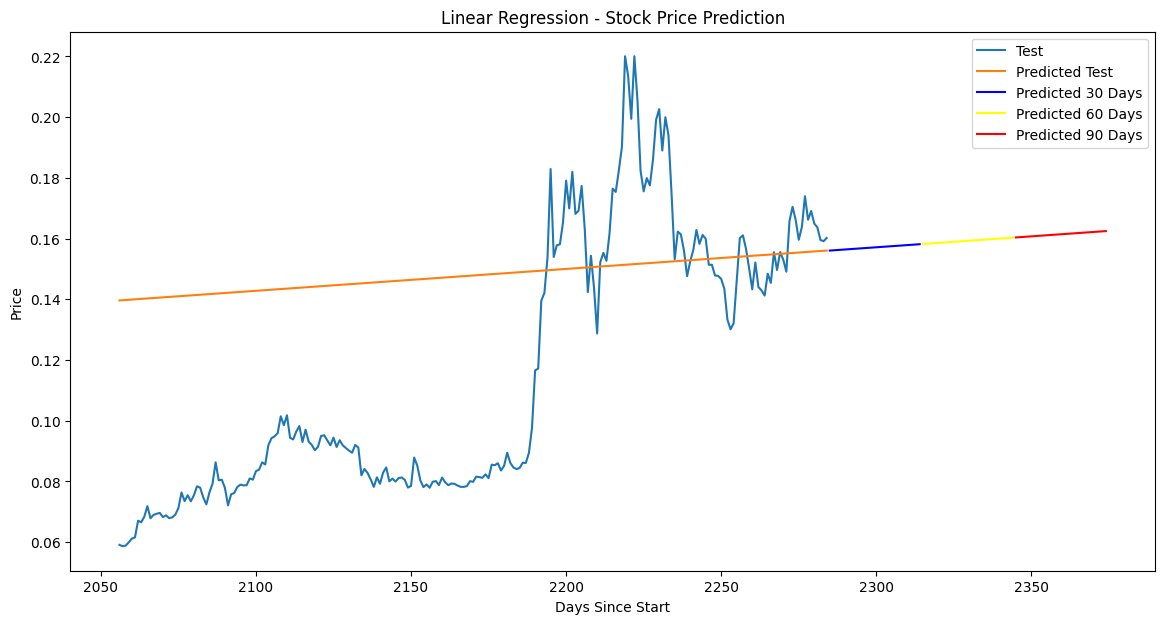
\includegraphics[width=1\textwidth]{bibliography/Figure/PREDICT/DOGE_LINEAR_9-1.png}
    \caption{Linear model's result with 9:1 splitting proportion}
    \label{fig10}
    \end{minipage}
    \hfill
    \begin{minipage}{0.23\textwidth}
    \centering
    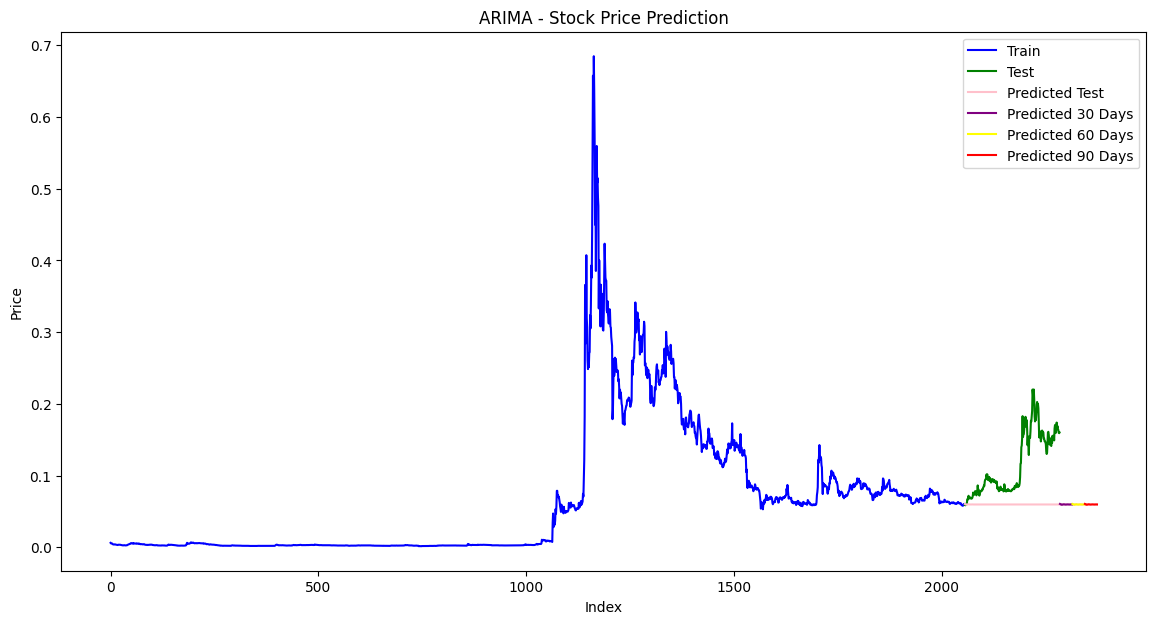
\includegraphics[width=1\textwidth]{bibliography/Figure/PREDICT/DOGE_ARIMA_9-1.png}
    \caption{ARIMA model's result with 9:1 splitting proportion}
    \label{fig11}
    \end{minipage}
\end{figure}

\begin{figure}[H]
    \centering
    \begin{minipage}{0.23\textwidth}
    \centering
    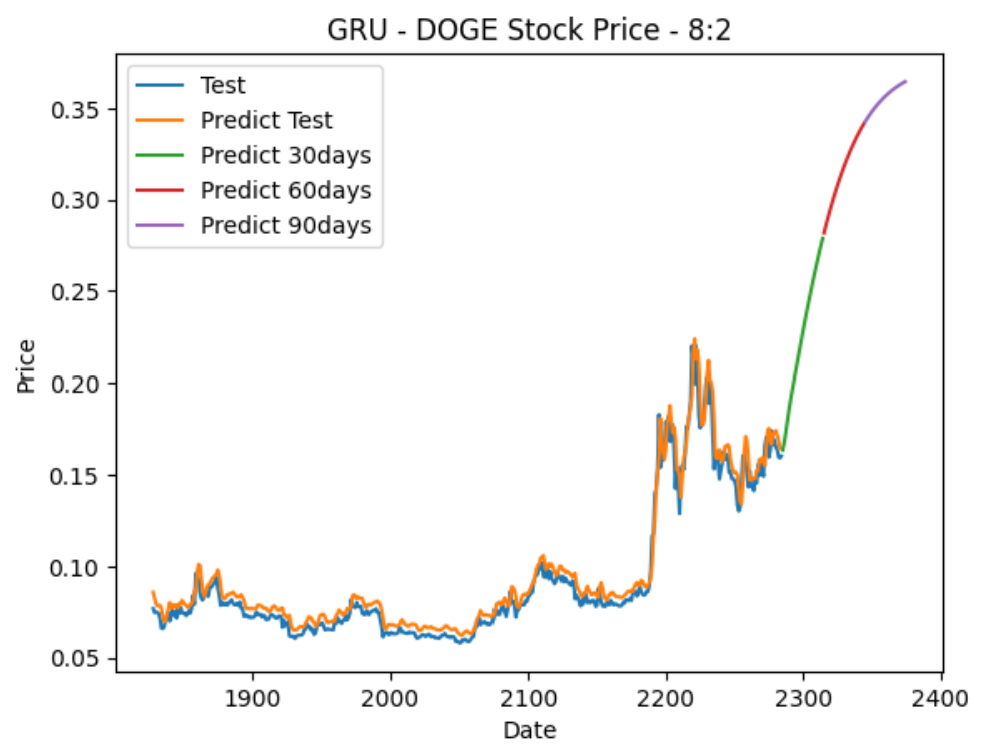
\includegraphics[width=1\textwidth]{bibliography/gru doge 82.png}
    \caption{GRU model's result with 8:2 splitting proportion}
    \label{fig10}
    \end{minipage}
    \hfill
    \begin{minipage}{0.23\textwidth}
    \centering
    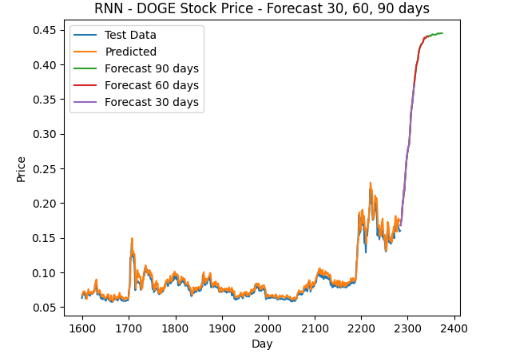
\includegraphics[width=1\textwidth]{bibliography/Figure/PREDICT/RNN/RNN-7-3-DOGE.png}
    \caption{RNN model's result with 7:3 splitting proportion}
    \label{fig11}
    \end{minipage}
\end{figure}

\begin{figure}[H]
    \centering
    \begin{minipage}{0.23\textwidth}
    \centering
    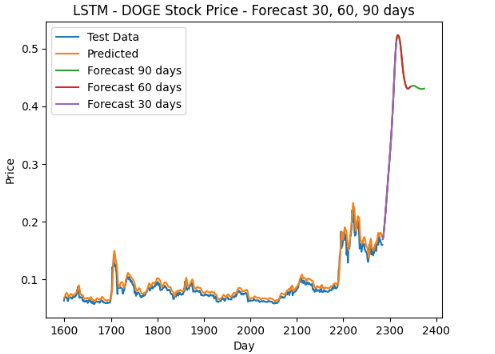
\includegraphics[width=1\textwidth]{bibliography/Figure/PREDICT/LSTM/LSTM-7-3-DOGE.png}
    \caption{LSTM model's result with 7:3 splitting proportion}
    \label{fig10}
    \end{minipage}
    \hfill
    \begin{minipage}{0.23\textwidth}
    \centering
    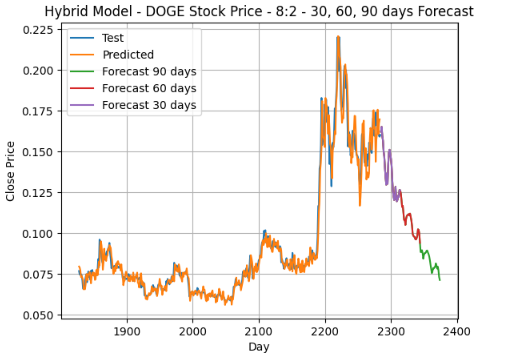
\includegraphics[width=1\textwidth]{bibliography/Figure/PREDICT/HYBRID MODELS/HB-8-2-DOGE.png}
    \caption{Hybrid Models's result with 8:2 splitting proportion}
    \label{fig11}
    \end{minipage}
\end{figure}

\begin{figure}[H]
    \centering
    \begin{minipage}{0.23\textwidth}
    \centering
    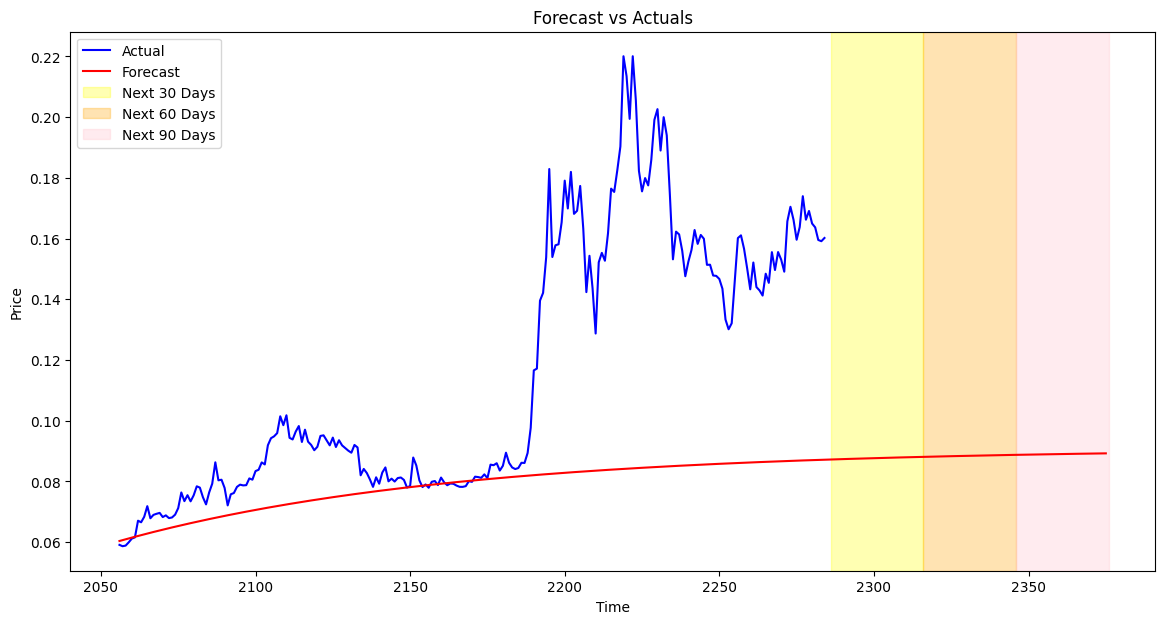
\includegraphics[width=1\textwidth]{bibliography/Figure/PREDICT/DOGE_AR-EMOS_9-1.png}
    \caption{AR-EMOS model's result with 9:1 splitting proportion}
    \label{fig10}
    \end{minipage}
    \hfill
    \begin{minipage}{0.23\textwidth}
    \centering
    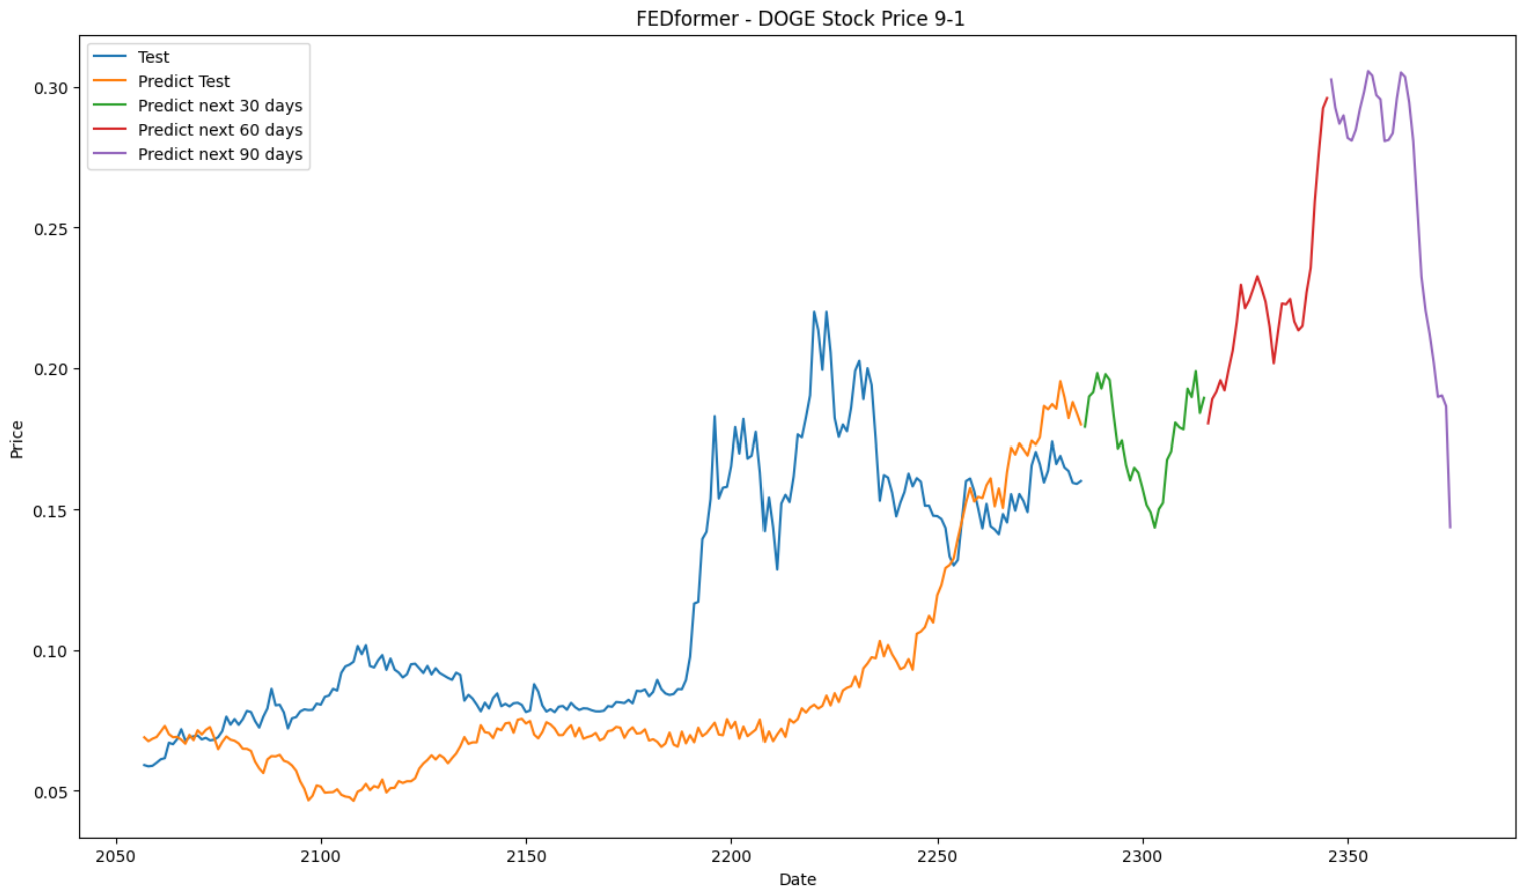
\includegraphics[width=1\textwidth]{bibliography/fed doge 91.png}
    \caption{FEDFORMER model's result with 9:1 splitting proportion}
    \label{fig11}
    \end{minipage}
\end{figure}
\subsection{ADA dataset} 
\begin{table}[H]
    \centering
    \begin{tabular}{|>{\centering\arraybackslash}p{1.1cm}|>{\centering\arraybackslash}p{1.8cm}|>{\centering\arraybackslash}p{1cm}|>{\centering\arraybackslash}p{1.3cm}|>{\centering\arraybackslash}p{1cm}|}
         \hline
         \multicolumn{5}{|c|}{\textbf{Dataset's Evaluation}}\\
        \hline
         Model & Training:Testing & MAE & RMSE & MAPE\\
         \hline
         \multirow{3}{*}{LN} & 7:3 & 1.193 & 1.4595 & 323.1359 \\ & 8:2 & 0.7622 & 0.591 & 209.98 \\ & \textbf{9:1} & \textbf{0.384} & \textbf{0.16} & \textbf{86.27} \\
         \hline
         \multirow{3}{*}{ARIMA} & 7:3 & 0.1097 & 0.0166 & 31.53 \\ & 8:2 & 0.1134 & 0.0219 & 25.188 \\ & \textbf{9:1} & \textbf{ 0.109} & \textbf{0.0166} & \textbf{31.53}\\
         \hline
         \multirow{3}{*}{GRU} & 7:3 &  0.2676 & 0.2789 & 207.0781 \\ &  8:2 & 0.2750 & 0.2890 & 209.5868 \\ & \textbf{9:1} & \textbf{0.0065} & \textbf{0.0087} & \textbf{4.0347}\\
         \hline
         \multirow{3}{*}{RNN} & 7:3 & 0.2650 & 0.2765 & 205.0486 \\ & \textbf{8:2} & \textbf{0.2597} & \textbf{0.2739} & \textbf{197.2246} \\ & 9:1 & 0.3563 & 0.3659 & 217.0752\\
         \hline
         \multirow{3}{*}{LSTM} & 7:3 & 0.2789 & 0.2897 & 216.9249 \\ & \textbf{8:2} & \textbf{0.2626} & \textbf{0.2772} & \textbf{199.1959} \\ &  9:1 & 0.3307 & 0.3403 & 200.8354\\
         \hline
         \multirow{3}{*}{\shortstack{HYBRID \\ MODELS}} & 7:3 & 0.0050 & 0.0069 & 3.7092\\ & \textbf{8:2} & \textbf{0.0048}	& \textbf{0.0069} & \textbf{3.4801}\\ & 9:1 & 0.0066 & 0.0089 & 3.9065\\
         \hline
         \multirow{3}{*}{AR-EMOS} & 7:3 &  0.23 & 0.067 & 69.368 \\ & 8:2 & 0.107 & 0.017 & 32.383 \\ & \textbf{9:1} &  \textbf{0.17848} &	\textbf{0.04325} & 	\textbf{32.0974} \\
         \hline
         \multirow{3}{*}{\shortstack{FED \\ FORMER}} & 7:3 & 4.0737 &  5.8607 &  935.2276 \\ & 8:2 & 0.4741 &  0.5943 &  108.5338 \\ & \textbf{9:1} & \textbf{0.2424} & \textbf{0.2720} & \textbf{44.1025}\\
         \hline
    \end{tabular}
    \caption{ADA Dataset's Evaluation}
    \label{mbbresult}
\end{table}

\begin{figure}[H]
    \centering
    \begin{minipage}{0.23\textwidth}
    \centering
    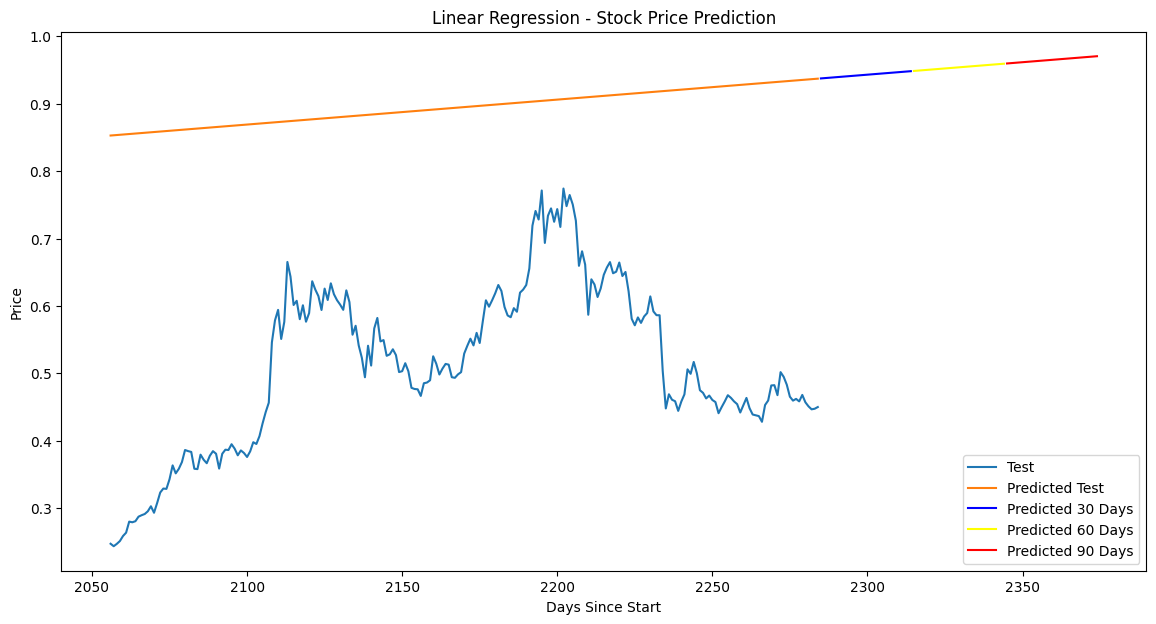
\includegraphics[width=1\textwidth]{bibliography/Figure/LINEAR_ADA_9-1.png}
    \caption{Linear model's result with 9:1 splitting proportion}
    \label{fig10}
    \end{minipage}
    \hfill
    \begin{minipage}{0.23\textwidth}
    \centering
    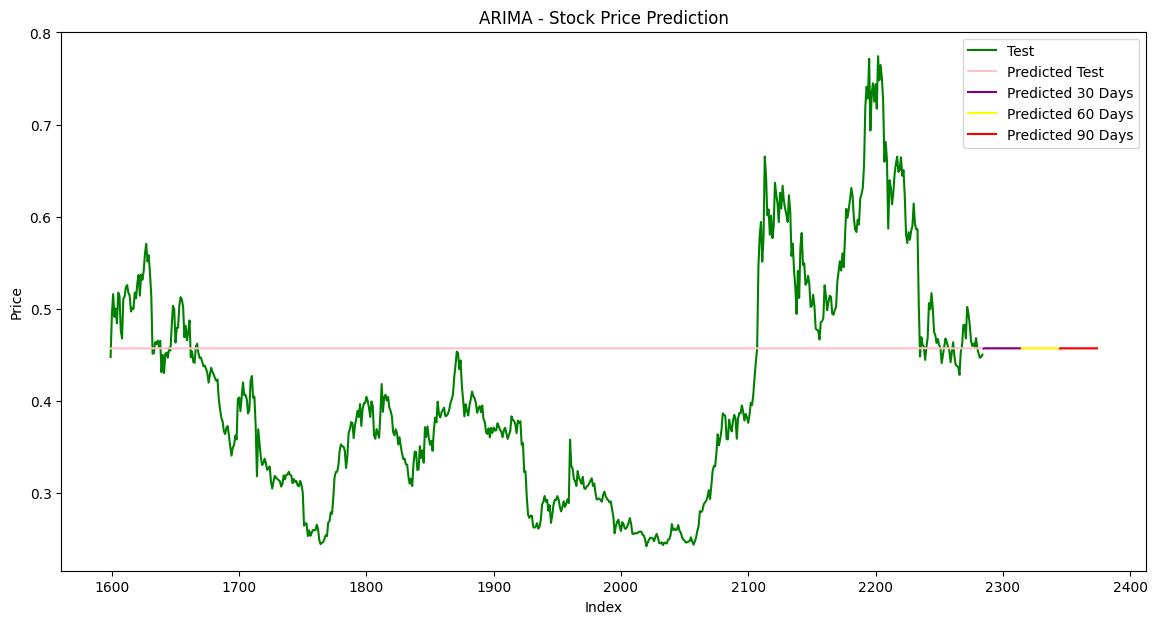
\includegraphics[width=1\textwidth]{bibliography/Figure/PREDICT/ADA_ARIMA_9-1.png}
    \caption{ARIMA model's result with 9:1 splitting proportion}
    \label{fig11}
    \end{minipage}
\end{figure}

\begin{figure}[H]
    \centering
    \begin{minipage}{0.23\textwidth}
    \centering
    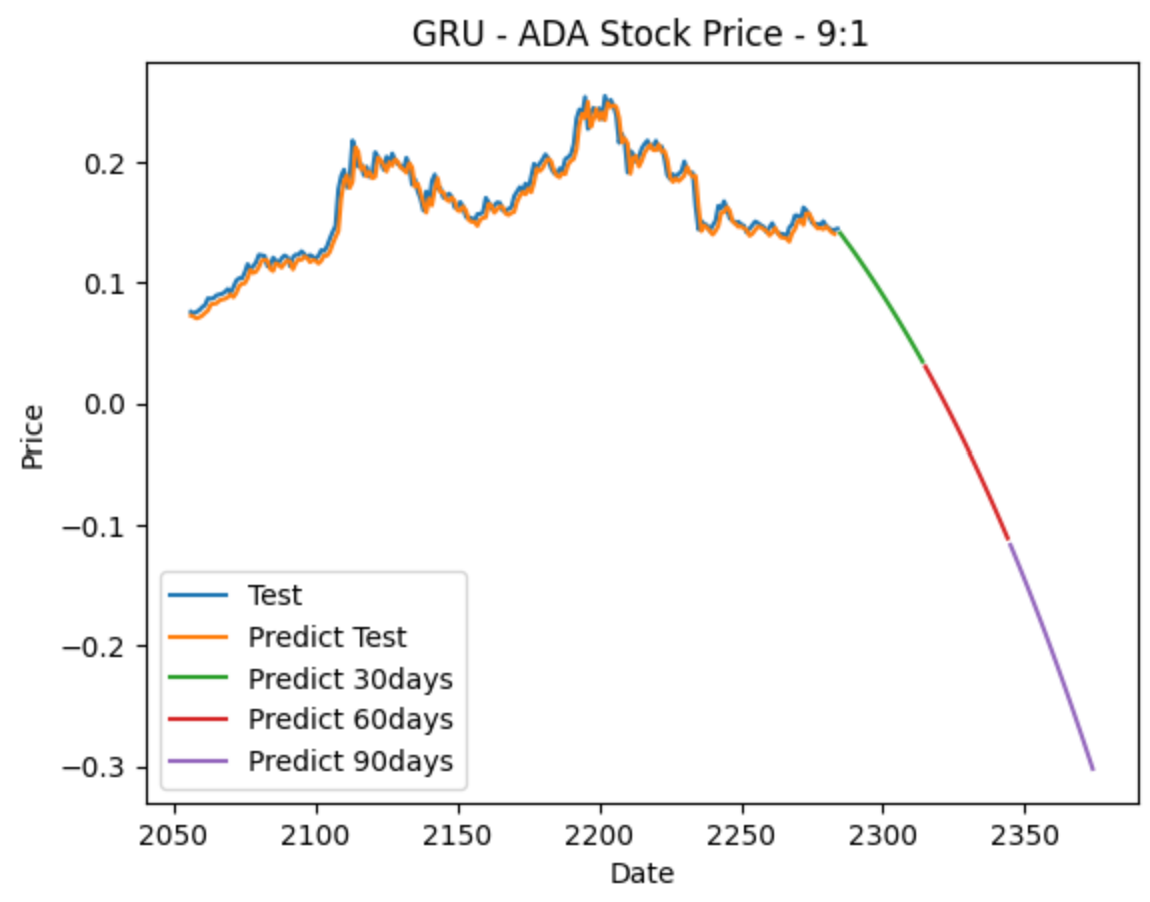
\includegraphics[width=1\textwidth]{bibliography/gru ada 91.png}
    \caption{GRU model's result with 9:1 splitting proportion}
    \label{fig10}
    \end{minipage}
    \hfill
    \begin{minipage}{0.24\textwidth}
    \centering
    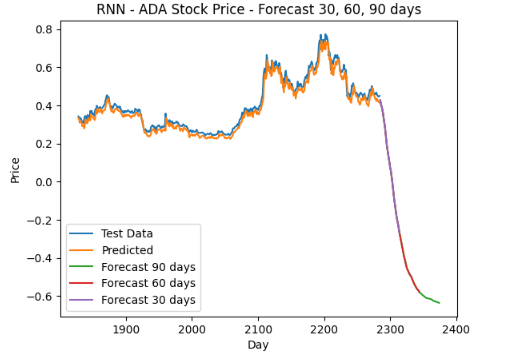
\includegraphics[width=1\textwidth]{bibliography/Figure/PREDICT/RNN/RNN-8-2-ADA.png}
    \caption{RNN model's result with 8:2 splitting proportion}
    \label{fig11}
    \end{minipage}
\end{figure}

\begin{figure}[H]
    \centering
    \begin{minipage}{0.23\textwidth}
    \centering
    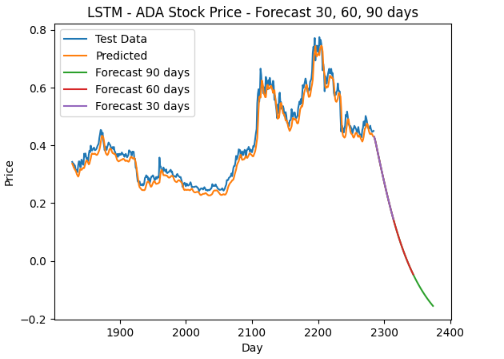
\includegraphics[width=1\textwidth]{bibliography/Figure/PREDICT/LSTM/LSTM-8-2-ADA.png}
    \caption{LSTM model's result with 8:2 splitting proportion}
    \label{fig10}
    \end{minipage}
    \hfill
    \begin{minipage}{0.23\textwidth}
    \centering
    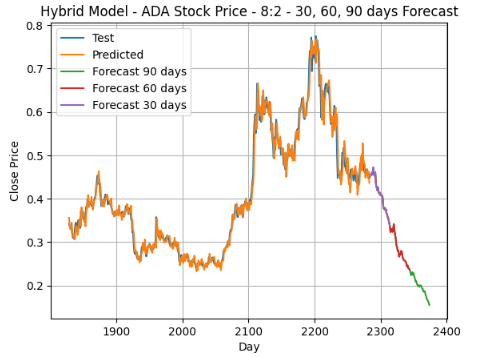
\includegraphics[width=1\textwidth]{bibliography/Figure/PREDICT/HYBRID MODELS/HB-8-2-ADA.png}
    \caption{Hybrid Models's result with 8:2 splitting proportion}
    \label{fig11}
    \end{minipage}
\end{figure}

\begin{figure}[H]
    \centering
    \begin{minipage}{0.23\textwidth}
    \centering
    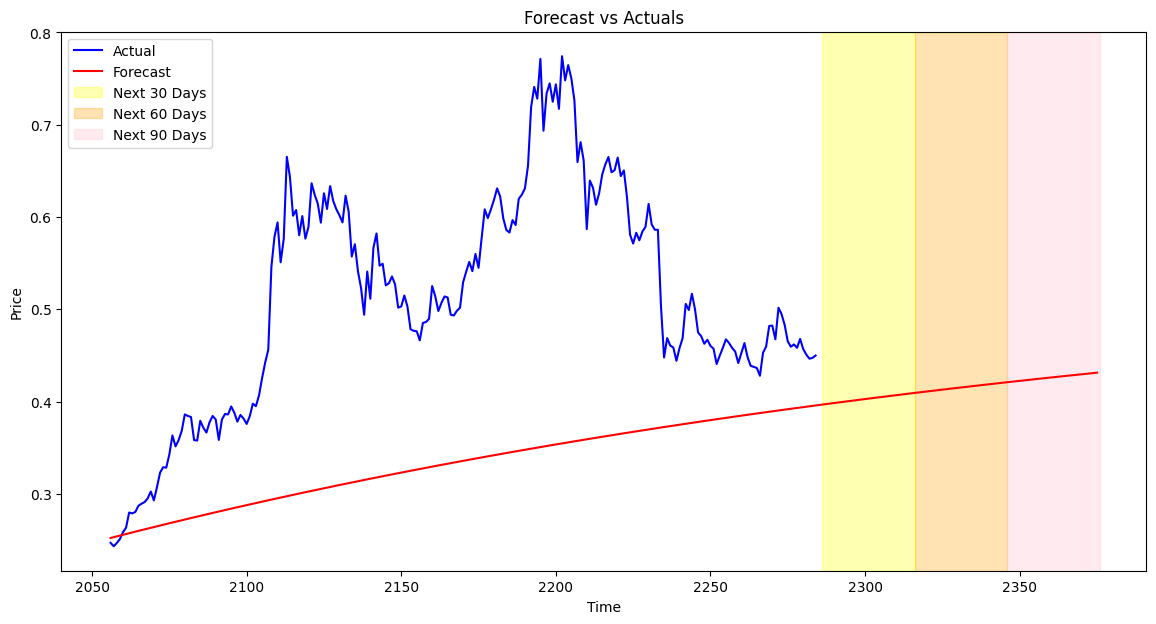
\includegraphics[width=1\textwidth]{bibliography/Figure/PREDICT/ADA_AR-EMOS_9-1.png}
    \caption{AR-EMOS model's result with 9:1 splitting proportion}
    \label{fig10}
    \end{minipage}
    \hfill
    \begin{minipage}{0.23\textwidth}
    \centering
    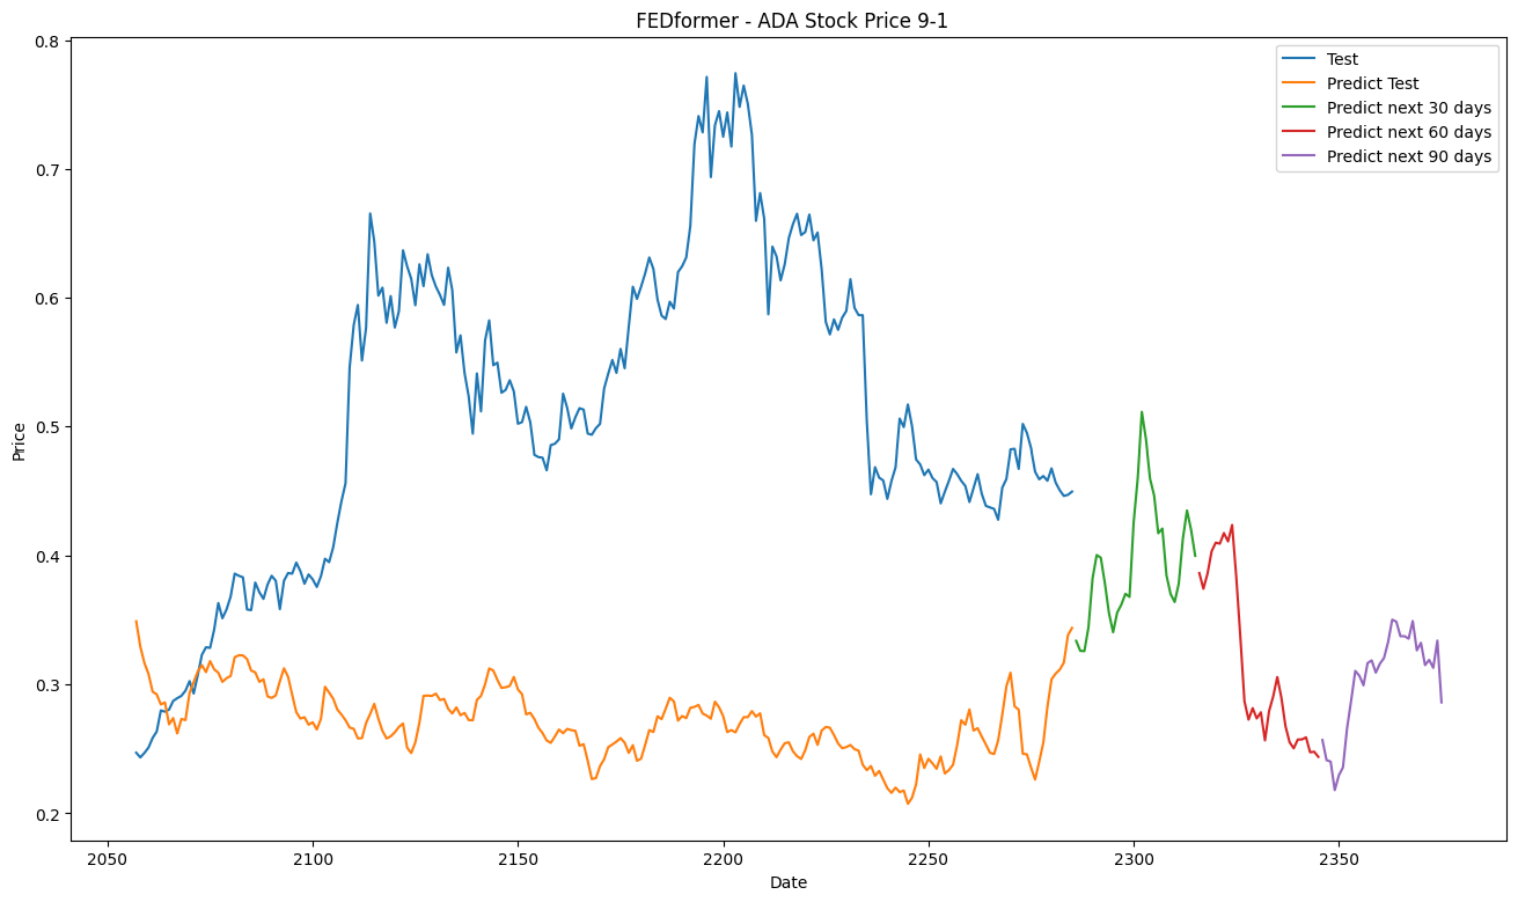
\includegraphics[width=1\textwidth]{bibliography/fed 91.png}
    \caption{FEDFORMER model's result with 9:1 splitting proportion}
    \label{fig11}
    \end{minipage}
\end{figure}
\section{Conclusion}
\subsection{Summary}
In the pursuit of forecasting cryptocurrency prices, a diverse array of methodologies has been explored, spanning from traditional statistical models to advanced machine learning algorithms. Among the models examined, including Auto Regressive Integrated Moving Average (ARIMA), Linear Regression (LR), Long Short-Term Memory (LSTM), Gated Recurrent Unit (GRU), Recurrent Neural Network (RNN), AR-EMOS, Hybrid Model, and FEDformer, it becomes apparent that certain models stand out for their predictive capabilities.\\
Cryptocurrency price forecasting, deeply rooted in the complexity and volatility of financial markets, requires models capable of capturing intricate patterns and relationships within the data. The GRU models, known for their proficiency in handling sequential dependencies, and the ensemble approaches like Hybrid Model and FEDformer, which leverage collective insights, demonstrate superior performance in predicting cryptocurrency prices.\\
Evaluation metrics, including RMSE, MAPE, and MSLE, consistently show that GRU, Hybrid Model, and FEDformer exhibit the highest forecasting accuracy across various metrics. These models' ability to adapt to the inherent uncertainties of cryptocurrency markets makes them invaluable tools for investors and analysts aiming for reliable predictions.
\subsection{Future Considerations}
Our future research should focus on optimizing the existing stock price prediction models by:
\\
\indent\textbullet\ 
Improving their accuracy: While the current models show promise, further refinement is needed to ensure more precise predictions.\\
\indent\textbullet\ Exploring alternative machine learning algorithms or ensemble techniques. Combining methods like multiple models or various ensemble learning approaches can also boost the robustness and accuracy of the forecasts.\\
\indent\textbullet\ Investigating new forecasting models: The field of forecasting is constantly evolving, and exploring new models with improved accuracy and performance is crucial.\\
By continuously incorporating new features, data sources, and modeling techniques, we can strive to optimize the forecasting models and enhance their ability to predict stock prices with greater precision and reliability.
\section*{Acknowledgment}
\addcontentsline{toc}{section}{Acknowledgment}
First and foremost, we would like to express our sincere gratitude to \textbf{Assoc. Prof. Dr. Nguyen Dinh Thuan} and \textbf{Mr. Nguyen Minh Nhut},  \textbf{Ms. Trinh Thi Thanh Truc}, \textbf{Ms. Dang Vu Phuong Uyen} for their exceptional guidance, expertise, and invaluable feedback throughout our research. Their mentorship and unwavering support have been crucial in shaping the direction and quality of this study. Their profound knowledge, critical insights, and attention to detail have greatly contributed to its success.
\\This research would not have been possible without their steadfast support and contributions. We sincerely thank everyone involved for their invaluable assistance, encouragement, and belief in our work.

%% UNCOMMENT these lines below (and remove the 2 commands above) if you want to embed the bibliografy.
\begin{thebibliography}{00}
\bibitem{b1} N. H. Gawali, “Bitcoin Price Prediction using Neural Network”.
\bibitem{b2} M. Ali and S. Shatabda, “A Data Selection Methodology to Train Linear Regression Model to Predict Bitcoin Price,” in 2020 2nd International Conference on Advanced Information and Communication Technology (ICAICT), Nov. 2020, pp. 330–335. doi: 10.1109/ICAICT51780.2020.9333525.
\bibitem{b3} P. Mondal, L. Shit, and S. Goswami, "Study of Effectiveness of Time Series Modeling (Arima) in Forecasting Stock Prices,"International Journal
of Computer Science, Engineering and Applications, vol. 4, no. 2, p. 13, Apr. 2014.
\bibitem{b4} M. Ridwan, K. Sadik, and F. M. Afendi, "Comparison of ARIMA and
GRU Models for High-Frequency Time Series Forecasting,"Scientific
Journal of Informatics, vol. 10, no. 3, pp. 389–400, Jan. 2024.
\bibitem{b5} M. Karim, M. Foysal, and S. Das, “Stock Price Prediction Using Bi-LSTM and GRU-Based Hybrid Deep Learning Approach,” Nov. 2022, pp. 701–711. doi: 10.1007/978-981-19-3148-2\_60.
\bibitem{b6} M. Bansal, A. Goyal, and A. Choudhary, “Stock Market Prediction with High Accuracy using Machine Learning Techniques,” Procedia Comput. Sci., vol. 215, pp. 247–265, Jan. 2022, doi: 10.1016/j.procs.2022.12.028.
\bibitem{b7} Vaddi, Lokesh. “Predicting Crypto Currency Prices Using Machine Learning and Deep Learning Techniques.” International Journal of Advanced Trends in Computer Science and Engineering 9, no. 4 (August 25, 2020): 6603–8. https://doi.org/10.30534/ijatcse/2020/351942020.

\bibitem{b8} M. Bansal, A. Goyal, and A. Choudhary, “Stock Market Prediction with High Accuracy using Machine Learning Techniques,” Procedia Comput. Sci., vol. 215, pp. 247–265, Jan. 2022, doi: 10.1016/j.procs.2022.12.028.

\bibitem{b9}  D. Montgomery, E. Peck, G. Vining, Introduction to linear regression analysis. John Wiley & Sons, 2021.

\bibitem{b10}
A. Ariyo, A. Adewumi, C. Ayo, "Stock price prediction using the ARIMA model," in 2014 UKSim-AMSS 16th international conference on computer modelling and simulation, 2014, pp. 106–112.

\bibitem{b11} C.-J. Chen, F.-I. Chou, and J.-H. Chou, “Temperature Prediction for Reheating Furnace by Gated Recurrent Unit Approach,” IEEE Access, vol. 10, pp. 33362–33369, 2022, doi: 10.1109/ACCESS.2022.3162424. [Accessed 20 May 2023].

\bibitem{b12} “10.2. Gated Recurrent Units (GRU) — Dive into Deep Learning documentation.” Available:  https://d2l.ai/chapter\_recurrent-modern/gru.html. [Accessed 27 May 2023].

\bibitem{b13} Encord, "Time series predictions with recurrent neural networks," Encord Blog. [Online]. Available: https://encord.com/blog/time-series-predictions-with-recurrent-neural-networks/. [Accessed: June 1, 2024].
\bibitem{b14} Anish Nama, "Understanding RNN (Recurrent Neural Network): Definition, Types, and Applications," Medium, April 21, 2023. [Online]. Available: https://medium.com/@anishnama20/understanding-rnn-recurrent-neural-network-definition-types-and-applications-3d57a80c0bc9. [Accessed: June 2, 2024].
\bibitem{b15} IBM, "Recurrent Neural Networks," IBM. [Online]. Available: https://www.ibm.com/topics/recurrent-neural-networks. [Accessed: June 18, 2024].
\bibitem{b16} Simplilearn, "LSTM Tutorial," Simplilearn. [Online]. Available: https://www.simplilearn.com/tutorials/artificial-intelligence-tutorial/lstm. Last updated: Apr 27, 2023. [Accessed: June 18, 2024].
\bibitem{b17} C. Olah, "Understanding LSTMs," Christopher Olah Blog, Aug. 27, 2015. [Online]. Available: https://colah.github.io/posts/2015-08-Understanding-LSTMs/. [Accessed: June 19, 2024].
\bibitem{b18} Ryan Holbrook, "Hybrid Models," Kaggle. [Online]. Available: https://www.kaggle.com/code/ryanholbrook/hybrid-models. [Accessed: June 1, 2024].
\bibitem{b19} X. Sha, "Time Series Stock Price Forecasting Based on Genetic Algorithm (GA)-Long Short-Term Memory Network (LSTM) Optimization," arXiv:2405.03151 [cs.LG], May 2024. [Online]. Available: https://arxiv.org/abs/2405.03151. [Accessed: June 20, 2024].

\bibitem{b20}D. Jobst, A. Moller, J. Groß. "Time Series based Ensemble Model Output Statistics for Temperature Forecasts Postprocessing," in arXiv preprint arXiv:2402.00555, 2024.

\bibitem{b21}  Gneiting, T., et al. "Calibrated probabilistic forecasting using ensemble model output statistics and minimum CRPS estimation," in Monthly Weather Review, vol. 133, no. 5, pp. 1098–1118, 2005.

\bibitem{b22}T. Zhou, Z. Ma, Q. Wen, X. Wang, L. Sun, and R. Jin, "FEDformer: Frequency Enhanced Decomposed Transformer for Long-Term Series Forecasting," in Proc. 39th Int. Conf. Mach. Learn., PMLR 162, pp. 27268-27286, 2022.

\bibitem{b23}A. Vaswani, N. Shazeer, N. Parmar, J. Uszkoreit, L. Jones, A. N. Gomez, Ł. Kaiser, and I. Polosukhin, "Attention is all you need," in Proc. 30th Int. Conf. Neural Inf. Process. Syst., Red Hook, NY, USA, pp. 6000–6010, 2017.


\end{thebibliography}
%%%%%%%%%%%%%%%


\EOD

\end{document}
